%%%%%%%%%%%%%%%%%%%%%%%%%%%%%%%%%%%%%%%%%
% Journal Article
% LaTeX Template
% Version 1.4 (15/5/16)
%
% This template has been downloaded from:
% http://www.LaTeXTemplates.com
%
% Original author:
% Frits Wenneker (http://www.howtotex.com) with extensive modifications by
% Vel (vel@LaTeXTemplates.com)
%
% License:
% CC BY-NC-SA 3.0 (http://creativecommons.org/licenses/by-nc-sa/3.0/)
%
%%%%%%%%%%%%%%%%%%%%%%%%%%%%%%%%%%%%%%%%%

%----------------------------------------------------------------------------------------
%	PACKAGES AND OTHER DOCUMENT CONFIGURATIONS
%----------------------------------------------------------------------------------------

\documentclass[twoside,twocolumn]{article}
%\usepackage[svgnames]{xcolor}


\usepackage{blindtext} % Package to generate dummy text throughout this template 

\usepackage[sc]{mathpazo} % Use the Palatino font
\usepackage[T1]{fontenc} % Use 8-bit encoding that has 256 glyphs
\linespread{1.05} % Line spacing - Palatino needs more space between lines
\usepackage{microtype} % Slightly tweak font spacing for aesthetics

\usepackage[british]{babel}

\usepackage[hmarginratio=1:1,top=32mm,columnsep=20pt]{geometry} % Document margins
\usepackage[hang, small,labelfont=bf,up,textfont=it,up]{caption} % Custom captions under/above floats in tables or figures
\usepackage{booktabs} % Horizontal rules in tables
\usepackage{floatrow}

\usepackage{lettrine} % The lettrine is the first enlarged letter at the beginning of the text

\usepackage[dvipsnames]{xcolor}
\usepackage[utf8]{inputenc}
%\usepackage[T1]{fontenc}
\usepackage{graphicx}
\usepackage[pages=some]{background}
\usepackage[nottoc]{tocbibind}
\usepackage{amssymb}
\usepackage{pifont}% http://ctan.org/pkg/pifont
\usepackage{tabularx, booktabs, makecell, caption}
 \usepackage{siunitx}
\usepackage{fancyhdr}
\usepackage{grffile}
\usepackage{cite}
\usepackage{subcaption}
\usepackage{adjustbox}
\usepackage{listings}
%\usepackage{float}
\usepackage{lscape}
\usepackage{tikz}
\usetikzlibrary{bayesnet}
\usetikzlibrary{arrows}
\usepackage{wrapfig}
\usepackage{cmap}
\usepackage{iflang}
\usepackage{multirow}
\usepackage{bm}
\usepackage{fancyvrb}
\usepackage[autostyle]{csquotes}
\usepackage{hyperref}
\usepackage{nomencl}
\usepackage{rotating}
\usepackage{ragged2e}
\usepackage{changepage}
\usepackage{setspace}
\usepackage{xargs}   
\usepackage[colorinlistoftodos,prependcaption,textsize=tiny]{todonotes}
\usepackage{algorithmicx}
\usepackage{algorithm}% http://ctan.org/pkg/algorithm
\usepackage{algpseudocode}% http://ctan.org/pkg/algorithmicx
%\usepackage{enumerate}% http://ctan.org/pkg/enumerate
\usepackage{xfrac}
\usetikzlibrary{arrows.meta,arrows}


\usepackage{enumitem} % Customized lists
\setlist[itemize]{noitemsep} % Make itemize lists more compact

\usepackage{abstract} % Allows abstract customization
\renewcommand{\abstractnamefont}{\normalfont\bfseries} % Set the "Abstract" text to bold
\renewcommand{\abstracttextfont}{\normalfont\small\itshape} % Set the abstract itself to small italic text

\usepackage{titlesec} % Allows customization of titles
\renewcommand\thesection{\Roman{section}} % Roman numerals for the sections
\renewcommand\thesubsection{\roman{subsection}} % roman numerals for subsections
\titleformat{\section}[block]{\large\scshape\centering}{\thesection.}{1em}{} % Change the look of the section titles
\titleformat{\subsection}[block]{\large}{\thesubsection.}{1em}{} % Change the look of the section titles

\renewcommand{\algorithmicrequire}{\textbf{Input:}}
\renewcommand{\algorithmicensure}{\textbf{Output:}}

\newcommand{\chapquote}[3]{\begin{quotation} \textit{#1} \end{quotation} \begin{flushright} -- #2, \textit{#3}\end{flushright} }
\definecolor{dkgreen}{rgb}{0,0.6,0}
\definecolor{gray}{rgb}{0.5,0.5,0.5}
\definecolor{mauve}{rgb}{0.58,0,0.82}



\newcommand\myshade{85}
\colorlet{mylinkcolor}{violet}
\colorlet{mycitecolor}{YellowOrange}
\colorlet{myurlcolor}{Aquamarine}

\hypersetup{
  linkbordercolor  = mylinkcolor!\myshade!black,
  citebordercolor  = mycitecolor!\myshade!black,
  urlbordercolor   = myurlcolor!\myshade!black,
}



\lstset{ %
  language=R,                     % the language of the code
  basicstyle=\footnotesize,       % the size of the fonts that are used for the code
  numbers=left,                   % where to put the line-numbers
  numberstyle=\tiny\color{gray},  % the style that is used for the line-numbers
  stepnumber=1,                   % the step between two line-numbers. If it's 1, each line
                                  % will be numbered
  numbersep=5pt,                  % how far the line-numbers are from the code
  %backgroundcolor=\color{white},  % choose the background color. You must add \usepackage{color}
  showspaces=false,               % show spaces adding particular underscores
  showstringspaces=false,         % underline spaces within strings
  showtabs=false,                 % show tabs within strings adding particular underscores
  %frame=single,                   % adds a frame around the code
  %rulecolor=\color{black},        % if not set, the frame-color may be changed on line-breaks within not-black text (e.g., commens (green here))
  tabsize=2,                      % sets default tabsize to 2 spaces
  captionpos=b,                   % sets the caption-position to bottom
  breaklines=true,                % sets automatic line breaking
  breakatwhitespace=false,        % sets if automatic breaks should only happen at whitespace
  title=\lstname,                 % show the filename of files included with \lstinputlisting;
                                  % also try caption instead of title
  keywordstyle=\color{blue},      % keyword style
  commentstyle=\color{dkgreen},   % comment style
  stringstyle=\color{mauve},      % string literal style
  escapeinside={\%*}{*)},         % if you want to add a comment within your code
  morekeywords={*,...}            % if you want to add more keywords to the set
} 



\newcommand{\otfrac}[2]{%
    \frac%
        {\raisebox{-.1em}{\scriptsize $#1$}}%
        {\raisebox{.15em}{\scriptsize $#2$}}%
}

\newcommandx{\unsure}[2][1=]{\todo[linecolor=red, backgroundcolor=white, bordercolor=red, #1]{#2}}
%\newcommandx{\change}[2][1=]{\todo[linecolor=blue,backgroundcolor=white,bordercolor=blue,#1]{#2}}
\newcommandx{\info}[2][1=]{\todo[linecolor=OliveGreen,backgroundcolor=white,bordercolor=OliveGreen,#1]{#2}}
\newcommandx{\improvement}[2][1=]{\todo[linecolor=Plum,backgroundcolor=white,bordercolor=Plum,#1]{#2}}
\newcommandx{\thiswillnotshow}[2][1=]{\todo[disable,#1]{#2}}
\newcommandx{\change}[2][1=]{\todo[disable,#1]{#2}}

\newcommand{\cmark}{\ding{51}}%
\newcommand{\xmark}{\ding{55}}%

\usepackage{fancyhdr} % Headers and footers
\pagestyle{fancy} % All pages have headers and footers
\fancyhead{} % Blank out the default header
\fancyfoot{} % Blank out the default footer
\fancyhead[C]{Preliminary Results \quad $\bullet$\quad Causal Bayesian networks \quad $\bullet$ \quad LMU Munich \quad $\bullet$\quad  \today} % Custom header text
\fancyfoot[RO,LE]{\thepage} % Custom footer text

\usepackage{titling} % Customizing the title section

\usepackage{hyperref} % For hyperlinks in the PDF

\usepackage{url}
\usepackage{grffile}

\usepackage{subcaption}
\usepackage{graphicx}
\usepackage{float}
\usepackage{wrapfig}

%----------------------------------------------------------------------------------------
%	TITLE SECTION
%----------------------------------------------------------------------------------------

\setlength{\droptitle}{-4\baselineskip} % Move the title up

\pretitle{\begin{center}\Huge\bfseries} % Article title formatting
\posttitle{\end{center}} % Article title closing formatting
\title{How the `fear factor' spreads across the global financial markets} % Article title
\author{%
\textsc{Jonas Gottal}\\[1ex] % Your name
\normalsize Preliminary results\thanks{Code available on GitHub:  \url{github.com}} of upcoming thesis at \\\normalsize Faculty of Mathematics, Computer Science and Statistics, \\\normalsize  Ludwig Maximilian University of Munich% Your institution
%\normalsize \href{mailto:john@smith.com}{john@smith.com} % Your email address
%\and % Uncomment if 2 authors are required, duplicate these 4 lines if more
%\textsc{Jane Smith}\thanks{Corresponding author} \\[1ex] % Second author's name
%\normalsize University of Utah \\ % Second author's institution
%\normalsize \href{mailto:jane@smith.com}{jane@smith.com} % Second author's email address
}
\date{15. Juli 2021} % Leave empty to omit a date
\renewcommand{\maketitlehookd}{%
\begin{abstract}
\noindent This excerpt serves as a summary of the application results of the underlying work as an attachment to the published code on GitHub. To apply our obtained knowledge described in the underlying thesis, we propose a use case in finance with real world data. Our interest targets  \textit{Implied Volatility} data and the relationships of this indicator between different countries. Since this measure is often used to capture the market's sentiment towards the volatility of a particular asset, it is also referred to as the ``fear factor''.  \cite{Joshi2008}  \cite{Hull2021}
\end{abstract}
}

%----------------------------------------------------------------------------------------

\begin{document}

% Print the title
\maketitle

%----------------------------------------------------------------------------------------
%	ARTICLE CONTENTS
%----------------------------------------------------------------------------------------
\section{Introduction}
The underlying thesis describes how agents can learn from data through probability theory by reformulating the task as exact inference and maximum likelihood. We focus on learning Bayesian networks and show why they provide optimal predictions, solutions to overfitting and how they even handle decision making with incomplete data. And since Bayesian networks provide the potential for causal interpretations, we conclude with causal discovery.  
This excerpt serves as a summary of the application results and the approach we propose is structured as follows: First, we discuss the terminology of financial markets and then analyse and process our raw data. After learning our Bayesian networks, we validate their predictive properties and compare them appropriately. Finally we apply methods of causal discovery to infer the actual impact of countries.

\section{Terminology: Financial Markets and Derivatives}

Besides dark pools there are two different ways to conclude a transaction: over-the-counter (OTC) between two firms, and exchange trades. At exchanges for every transaction the order book is filled with the relevant (and thus for us useful) information, while OTC and dark pool trades remain invisible to the public eyes. We further separate between the stock market and derivatives market, which is significantly bigger in terms of underlying assets. By exploiting minuscule price differences on two or more exchanges to their own benefit, arbitrageurs balance these markets. Thus we can utilise the information from the derivative exchanges to gain insights into the stock market and vice versa. But what are derivatives? As an umbrella term, it is vaguely defined as an agreement between two parties on a future transaction, where the value can be \textit{derived} from a number of underlying variables. The two most popular derivatives are futures and options. While the future is a firm agreement to buy or sell an underlying asset \textit{at} a specified time in the \textit{future} at a specified price, the option gives the holder the right -- the \textit{option} -- to exercise the trade \textit{up to} the specified time. These options can now be used to calculate the so called \textit{implied volatility} -- volatility \textit{implied} by the option's prices.
And while calculating historical volatility -- via standard deviation -- is straight forward, the calculation of implied volatility is more complicated and not part of this thesis. For example the famous Black-Scholes approach aims to approximate the price of an option by modelling the geometric brownian motion -- taking into account for volatility, time and the current price of the underlying, among other variables. And if you apply this model in the opposite direction, you can calculate the implied volatility for the underlying using the current option prices. \cite{Joshi2008}  \cite{Hull2021} \\
Implied volatilities are calculated for countless financial products -- but our focus is on national equity market indices, replicating a countries stock market performance in one instrument. We gathered a data set of implied volatility indices from the twelve most important countries for financial markets, summarised in Table~\ref{tab:rawdata}.  Intraday data would be optimal to analyse the simultaneous changes on each exchange, but unfortunately, we were only able to collect daily data (end of day). However, for a long time horizon of up to 10 years.   \cite{Hull2021}

\section{Data Management: Preprocessing and Validation}
Our data set (Table~\ref{tab:rawdata}, Appendix) contains twelve different implied volatility indices, each replicating the implied volatility of national stock market indices.  For reasons of readability, we refer to them in the following by the name of the respective country. The raw time series of daily implied volatility in percent points (Figure~\ref{fig:timeseriesraw}) demonstrates an important property for our further analyses: stationarity. Thus, our means, variances, and correlations do not vary excessively and we do not have to address the influence of a global trend within our time series. Also within non-dynamic Bayesian networks the underlying generating process can not change over time and the predictive accuracy of our models would differ at different points in time. Obviously our data shows some outliers (especially Russia in 2014 due to oil prices) and trends at more granular level, but in general our data provides sufficient quality. \cite{Glymour2019} \cite{Shumway2017}
\begin{figure}[H]
\centering
% \begin{adjustwidth}{-0.25cm}{}
  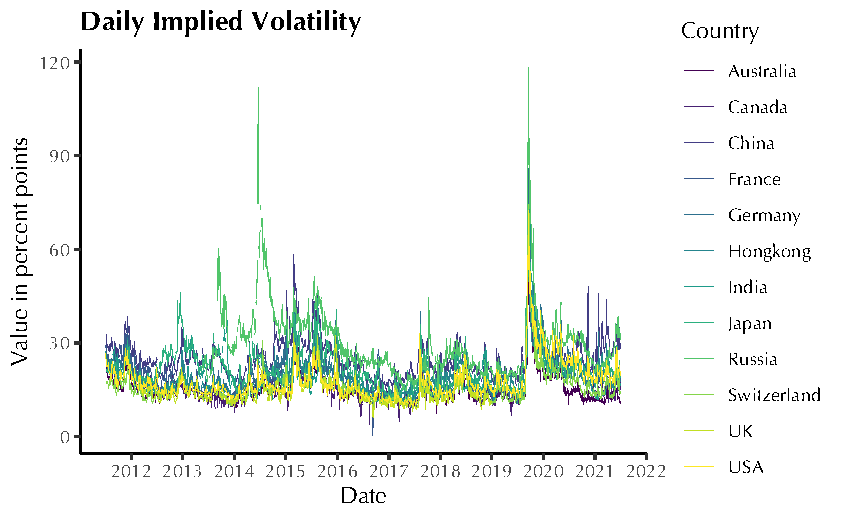
\includegraphics[trim={0 0 0 0},clip, width=1.0\linewidth]{../3. Code/Implied Volatility/Exports/Data/Timeseries1}
  \caption[Daily Implied Volatility]{Stationary time series: An index value of 30 means that the implied volatility of the underlying is considered to be at 30\%.}
  \label{fig:timeseriesraw}
  \end{figure}
  
But we care mostly about the daily changes while the different markets interact and therefor calculated them as daily \textit{log returns} for multiple reasons: The most important one is that a stock market can be approximated as a geometric Brownian motion and we can use \textit{It\^{o}'s lemma} to derive that they are log-normally distributed. And since we are aiming for normally distributed variables, we chose the natural logarithm to achieve this. Furthermore this approach yields a normalised data set (Figure~\ref{fig:timeseriesdaily}).  \cite{Joshi2008} \cite{Hull2021}



\begin{figure}[H]
\centering
  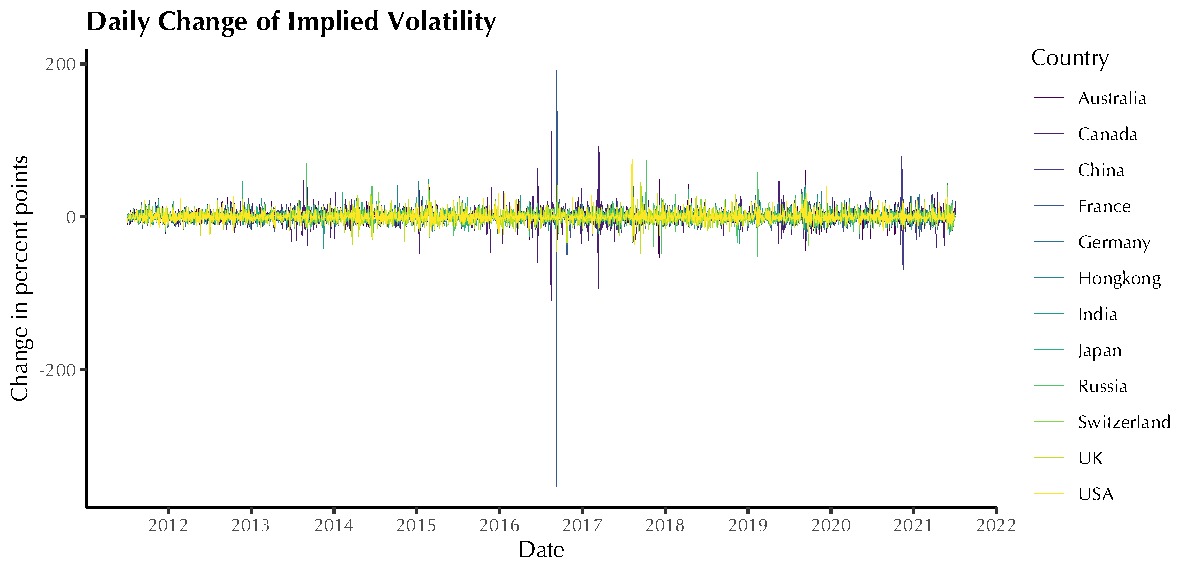
\includegraphics[trim={0 0 0 0},clip, width=1.0\linewidth]{../3. Code/Implied Volatility/Exports/Data/Timeseries2}
\caption[Change of daily Implied Volatility]{Daily log returns. }
  \label{fig:timeseriesdaily}
%   \end{adjustwidth}
\end{figure}

And since we want to analyse the impact of one country on another, but do not need to predict the exact value of the index, we are satisfied with the up- and downward movements. Thus, we discretise our data, with \texttt{1} representing positive and \texttt{-1}  negative changes. Due to the immense activity in these large financial instruments, there are no sideways movements and therefore no  values of \texttt{0}. As in Figure~\ref{fig:balanced} illustrated, the values are balanced and not skewed in either direction.

\begin{figure}[H]
\centering
  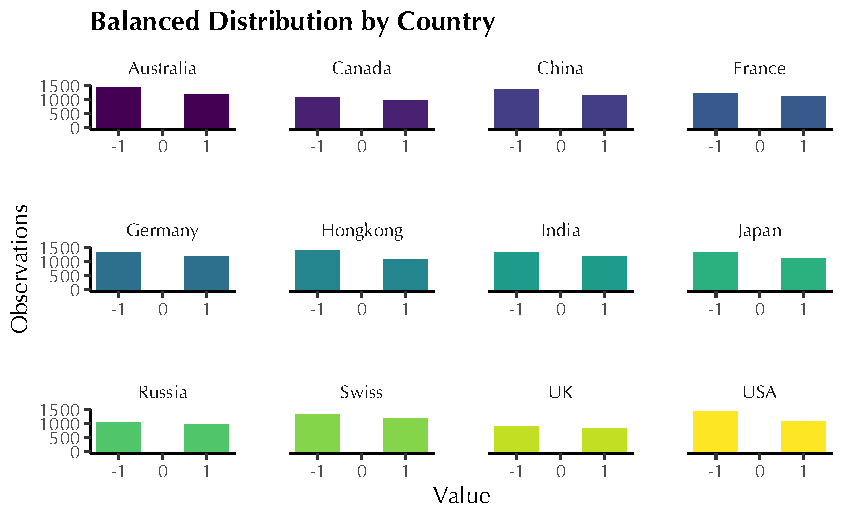
\includegraphics[trim={0 0 0 0},clip, width=1.0\linewidth]{../3. Code/Implied Volatility/Exports/Data/Distribution}
  \caption[Distribution of binary data]{  A balanced distribution between -1 and 1.}
  \label{fig:balanced}
\end{figure}
For validation purposes, we randomly split our dataset row-wise into a test  and  training set with the ratio \sfrac{1}{3} and \sfrac{2}{3}, leaving still enough data to train reliable models. For the EM algorithm we use the incomplete data as is, but for the score based approaches we omit the rows of the train set with missing values -- resulting in the EM algorithm seeing  more data. The test set for both is without rows of missing values and therefore the same to be comparable for subsequent validation. \cite{Kauermann2021} \cite{Hastie2009}


\section{Learning Networks from Implied Volatility Data}
With our processed and discretised data, we can now learn our Bayesian network's structure and parameters. Due to the diversity of algorithms and score functions in \texttt{bnlearn}, we have to make some restrictions. As previously discussed hybrid and constraint-based approaches perform less accurately. \cite{Scutari2019}  Therefore we only implemented three hybrid algorithms (\textit{Restricted Maximization, Hybrid HPC, Max-Min Hill-Climbing}) to verify this thesis for our data, but mostly focus on the score functions in Table~\ref{tab:score} optimised by Hill-Climbing and Tabu from prior sections. Furthermore we implement the EM algorithm from prior sections, with the maximisation step conducted by each Hill-Climbing and Tabu.

\begin{wrapfigure}[7]{r}{0.4\linewidth}
\begin{subfigure}{\linewidth}
  \centering
\begin{tikzpicture}[
  node distance=0.35cm and 0cm,
  mynode/.style={draw,circle,text width=0.15cm, align=center, fill=white},
  mycenter/.style={draw,circle,text width=0.15cm,align=center, fill=gray!30}
]
% nodes
%\node[mycenter] (n) {n}; %
 \node[mynode] (a) {\tiny{a}}; %
 \node[mynode,right=of a,xshift=0.5cm] (b) {\tiny{b}}; %
 \node[mynode,below=of b, xshift=-0.5cm] (c) {\tiny{c}}; %
% edges
 \draw[-{Latex[length=1.5mm, width=1mm]}] (b) -- (c);
 \draw[-{Latex[length=1.5mm, width=1mm]}] (a) -- (c);
 \end{tikzpicture}
 \end{subfigure}
 \caption[Markov Equivalence classes]{\small v-structure}
   \label{fig:vstructure}
\end{wrapfigure}


As the name suggests, information-theoretic scoring functions are based on information theory and often equivalent to a well established concept (e.g., BIC~$\Leftrightarrow$~MDL, Loglik~$\Leftrightarrow$~(cross)~entropy),  and Bayesian scoring functions utilise Bayes theorem and maximise the a-posteriori probability distribution of the networks. \cite{Carvalho2009} \cite{Scutari2022} 
\textit{Score-equivalence} means the scoring function assigns the same score to all networks in the same  \textit{Markov equivalence} class, denoted by the same conditional independencies. In general, these equivalence classes are Completed Partially Directed Acyclic Graphs (CPDAG) whose only directed arcs either belong to v-structures, as illustrated in Figure~\ref{fig:vstructure}, or would lead to another v-structure or cycle if reversed. We will learn more about them in Section~\ref{subsec:causal}. \cite{Nagarajan2014} \cite{Scutari2022} \cite{Castelletti2018}\\

To verify -- or exclude -- the presented scoring functions, as well as hybrid- and score-based algorithms, we run a $k$-fold cross validation to measure the loss of our data. This means we 
partition our data in $k$ equal-sized parts, and learn the model with $k-1$ parts. To validate them, we calculate the negated expected log-likelihood -- \textit{negative entropy} --  of the remaining partition $k$, where lower values are better. \cite{Nagarajan2014} \cite{Hastie2009} \cite{Scutari2022} The results in Figure~\ref{fig:loss} show, that we can not exclude certain combinations, as the overall loss is very similar.


\begin{figure}[H]
\centering
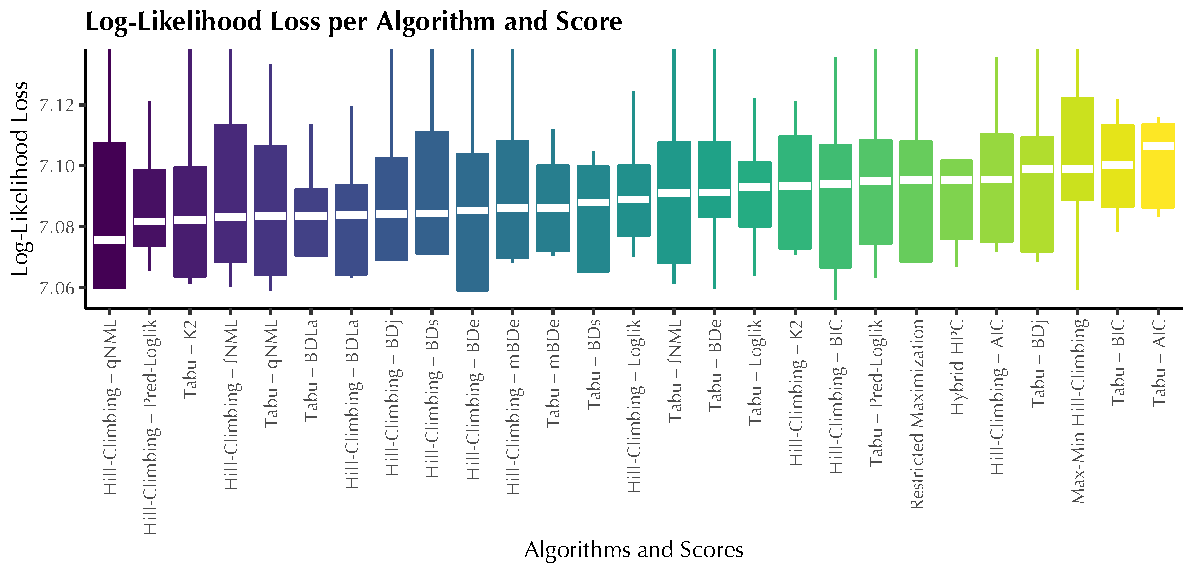
\includegraphics[trim={0 0 0 0},clip, width=1.0\linewidth]{../3. Code/Implied Volatility/Exports/Networks/Loss}
  \caption[$k$-fold cross validation]{$k$-fold cross validation with $k = 10$ folds to verify the fit of the algorithms and scoring functions to our data as implemented in R.}
  \label{fig:loss}
%   \end{adjustwidth}
\end{figure}

We apply both the score-based and hybrid approaches by averaging $n = 100$ networks of a bootstrap approach: by estimating the confidence in individual arcs and setting their minimum threshold, we obtain a more robust structure overall as implemented in \texttt{R}. ­­ The following networks in Figure~\ref{fig:bayesnets} are the results, but as they are differing in many arcs and orderings, we need to define a way to objectively validate and compare of our different models.\cite{Nagarajan2014}  \cite{Scutari2022}  \cite{Imoto2002} \cite{Friedman1999}



\begin{figure*}
\centering
   \scalebox{0.65}{
\begin{tabular}{cccc}
  \includegraphics[width=45mm]{../3. Code/Implied Volatility/Exports/Networks/Hill-Climbing – AIC} &  \includegraphics[width=45mm]{../3. Code/Implied Volatility/Exports/Networks/Tabu – AIC} &  \includegraphics[width=45mm]{../3. Code/Implied Volatility/Exports/Networks/Hill-Climbing – BIC} &  \includegraphics[width=45mm]{../3. Code/Implied Volatility/Exports/Networks/Tabu – BIC} \\
   \includegraphics[width=45mm]{../3. Code/Implied Volatility/Exports/Networks/Hill-Climbing – Loglik}& \includegraphics[width=45mm]{../3. Code/Implied Volatility/Exports/Networks/Tabu – Loglik} & \includegraphics[width=45mm]{../3. Code/Implied Volatility/Exports/Networks/Hill-Climbing – Pred-Loglik}&  \includegraphics[width=45mm]{../3. Code/Implied Volatility/Exports/Networks/Tabu – Pred-Loglik}\\

\includegraphics[width=45mm]{../3. Code/Implied Volatility/Exports/Networks/Hill-Climbing – fNML}& \includegraphics[width=45mm]{../3. Code/Implied Volatility/Exports/Networks/Tabu – fNML} &\includegraphics[width=45mm]{../3. Code/Implied Volatility/Exports/Networks/Hill-Climbing – qNML} &\includegraphics[width=45mm]{../3. Code/Implied Volatility/Exports/Networks/Tabu – qNML}\\

 \includegraphics[width=45mm]{../3. Code/Implied Volatility/Exports/Networks/Hill-Climbing – BDe} &\includegraphics[width=45mm]{../3. Code/Implied Volatility/Exports/Networks/Tabu – BDe}&    \includegraphics[width=45mm]{../3. Code/Implied Volatility/Exports/Networks/Hill-Climbing – BDj} & \includegraphics[width=45mm]{../3. Code/Implied Volatility/Exports/Networks/Tabu – BDj}\\

    \includegraphics[width=45mm]{../3. Code/Implied Volatility/Exports/Networks/Hill-Climbing – BDLa} &\includegraphics[width=45mm]{../3. Code/Implied Volatility/Exports/Networks/Tabu – BDLa} &    \includegraphics[width=45mm]{../3. Code/Implied Volatility/Exports/Networks/Hill-Climbing – BDs} &\includegraphics[width=45mm]{../3. Code/Implied Volatility/Exports/Networks/Tabu – BDs} \\

 \includegraphics[width=45mm]{../3. Code/Implied Volatility/Exports/Networks/Hill-Climbing – mBDe} &\includegraphics[width=45mm]{../3. Code/Implied Volatility/Exports/Networks/Tabu – mBDe} &     \includegraphics[width=45mm]{../3. Code/Implied Volatility/Exports/Networks/Hill-Climbing – K2}  & \includegraphics[width=45mm]{../3. Code/Implied Volatility/Exports/Networks/Tabu – K2}\\

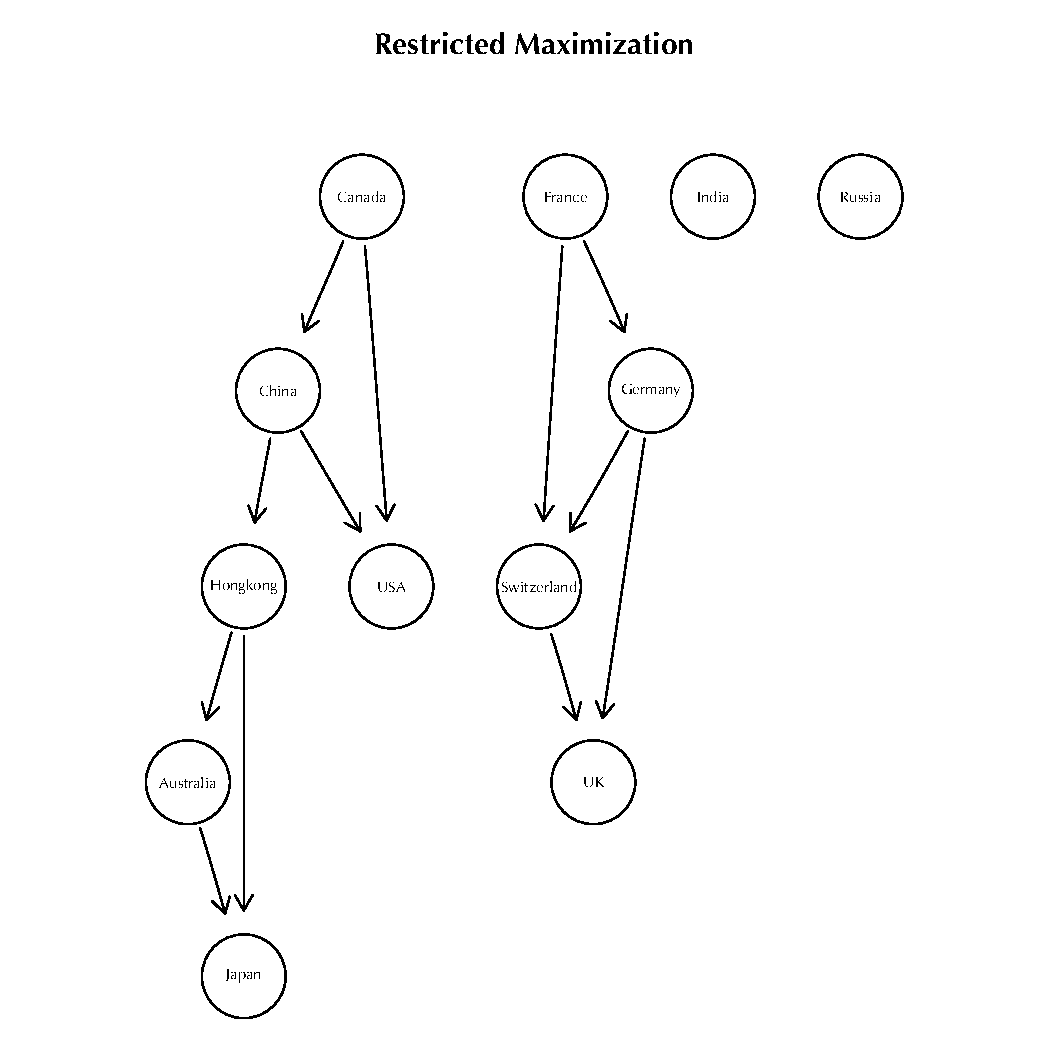
\includegraphics[width=45mm]{../3. Code/Implied Volatility/Exports/Networks/Restricted Maximization} &  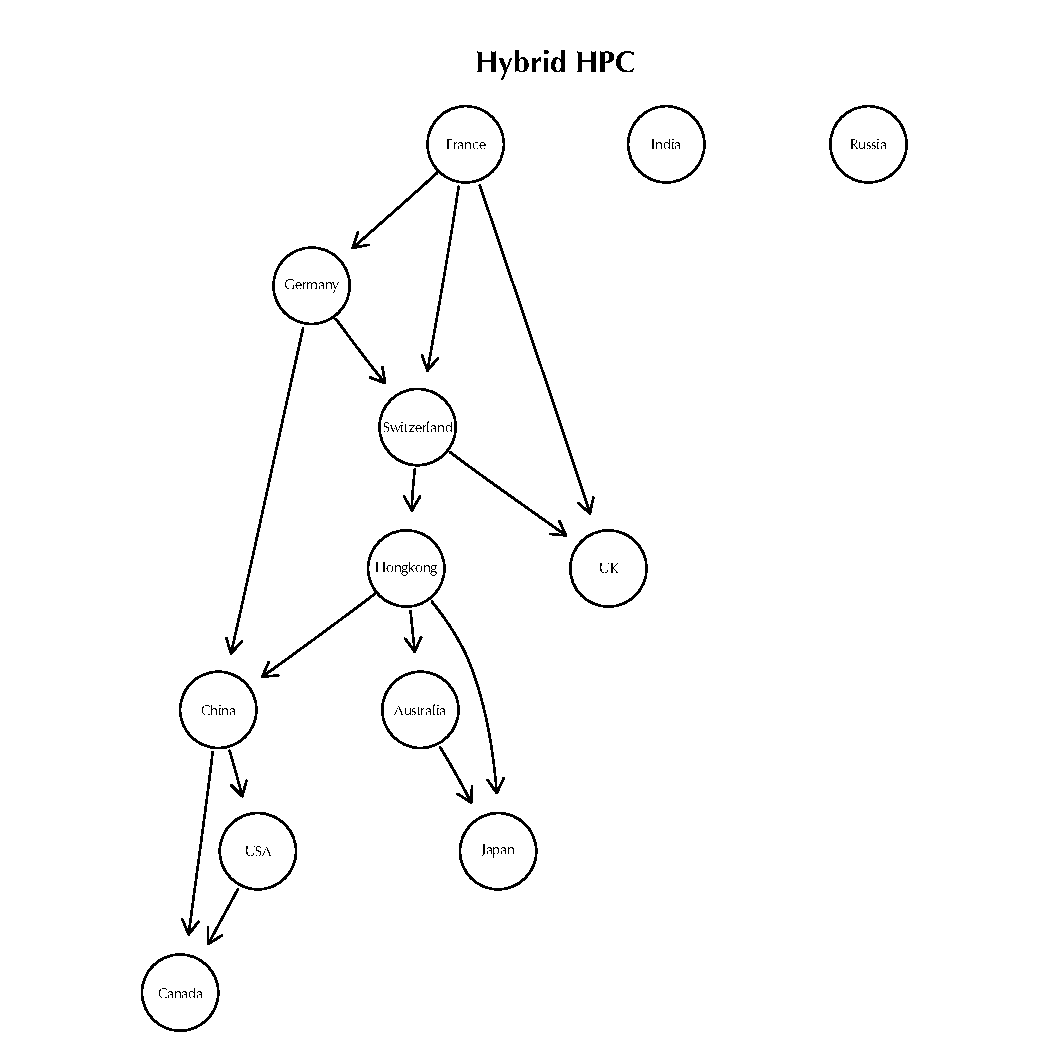
\includegraphics[width=45mm]{../3. Code/Implied Volatility/Exports/Networks/Hybrid HPC} &  \includegraphics[width=45mm]{../3. Code/Implied Volatility/Exports/Networks/EM – Hill-Climbing} & \includegraphics[width=45mm]{../3. Code/Implied Volatility/Exports/Networks/EM – Tabu}  \\
\end{tabular}
}
\caption[Overview of all learned Bayesian networks]{Resulting learned Bayesian networks with dedicated algorithms and scoring functions}
  \label{fig:bayesnets}
\end{figure*}


\begin{figure*}
\begin{tabular}{cccc}
  
\includegraphics[width=45mm]{../3. Code/Implied Volatility/Exports/ROC/Australia} &   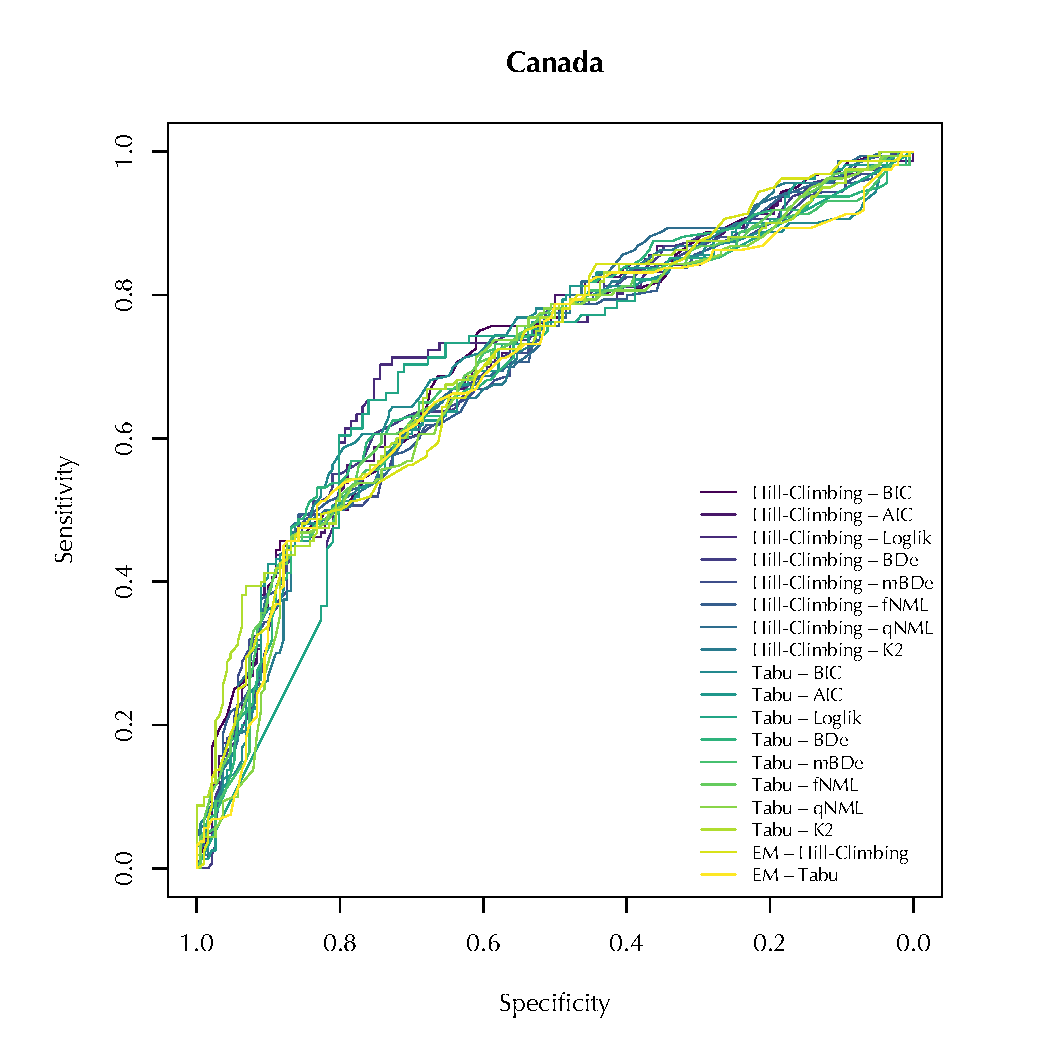
\includegraphics[width=45mm]{../3. Code/Implied Volatility/Exports/ROC/Canada} &    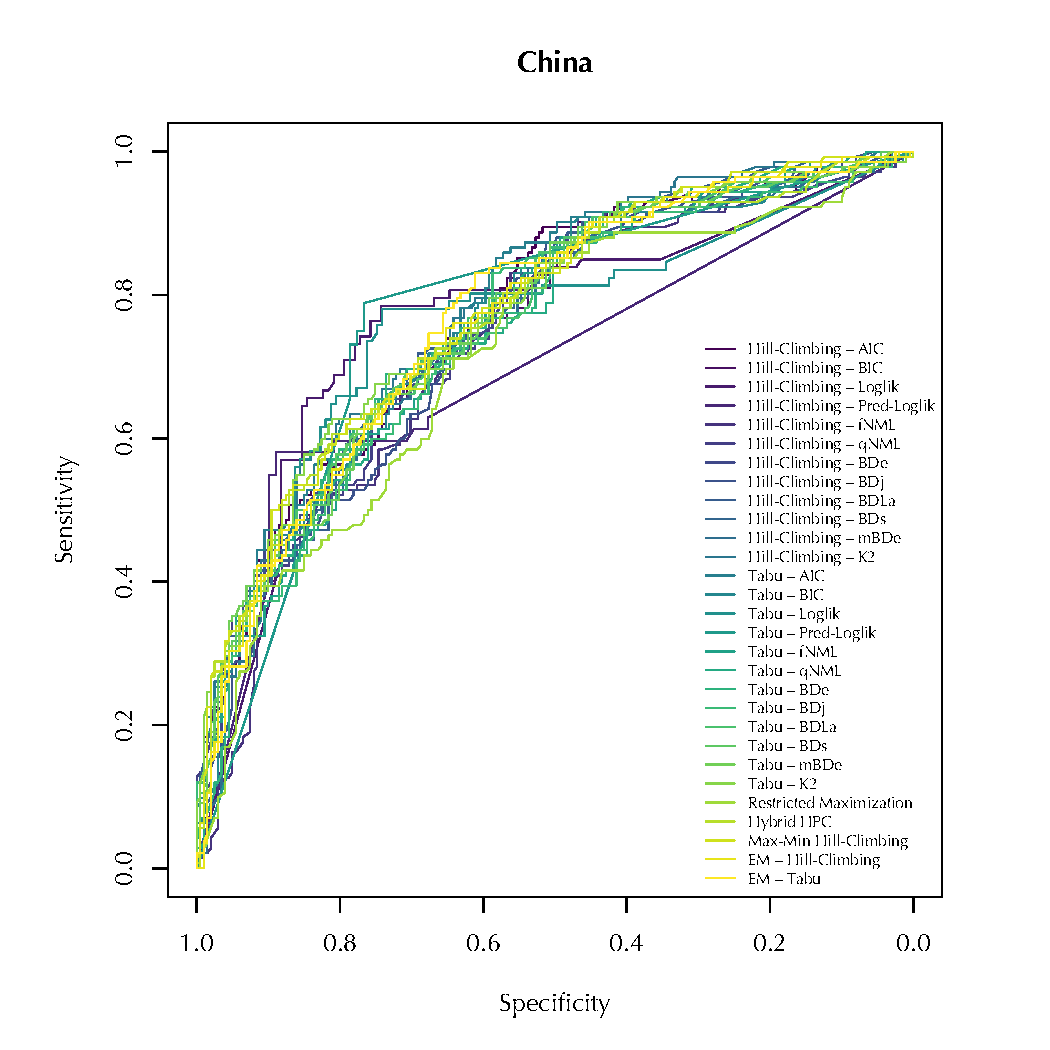
\includegraphics[width=45mm]{../3. Code/Implied Volatility/Exports/ROC/China}  \\ 
\includegraphics[width=45mm]{../3. Code/Implied Volatility/Exports/ROC/France} &      
\includegraphics[width=45mm]{../3. Code/Implied Volatility/Exports/ROC/Germany} &  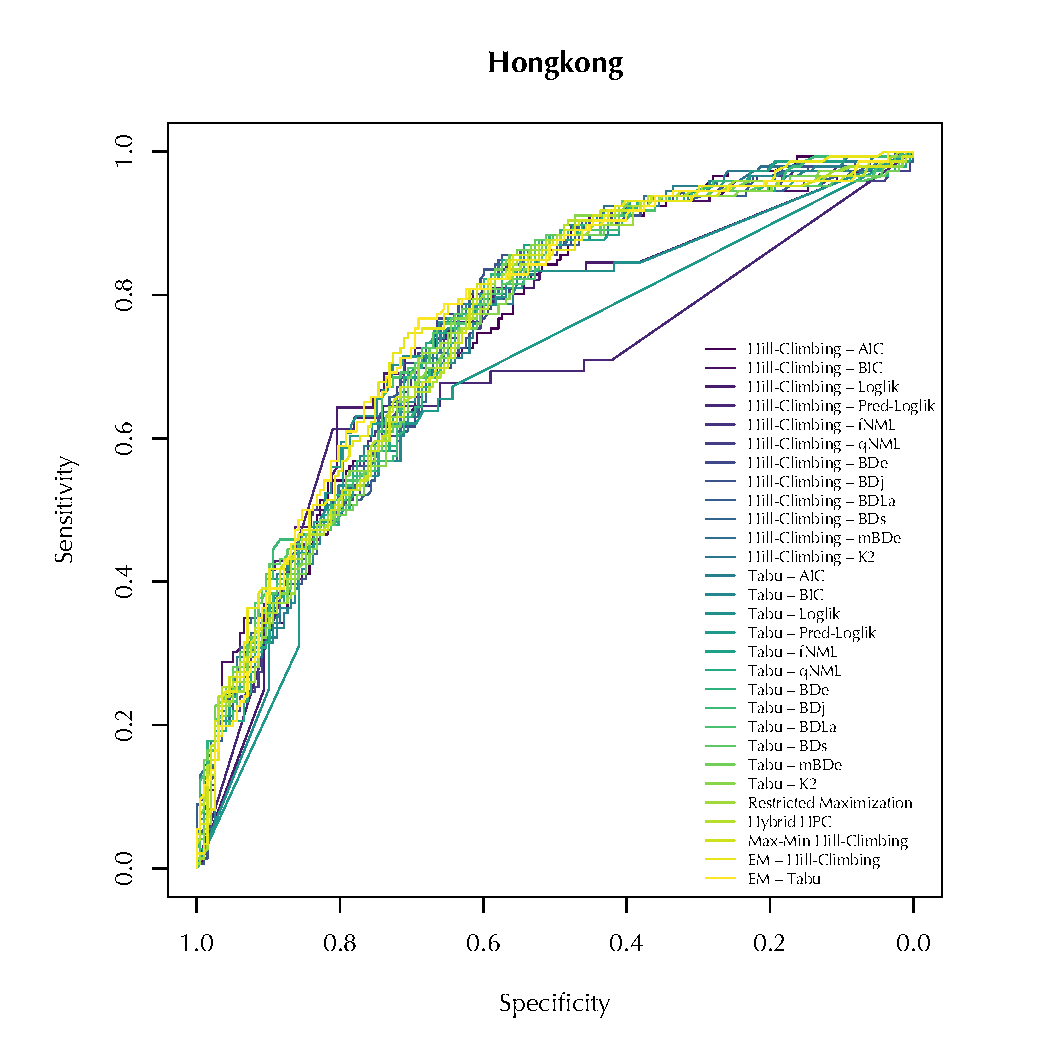
\includegraphics[width=45mm]{../3. Code/Implied Volatility/Exports/ROC/Hongkong}  \\  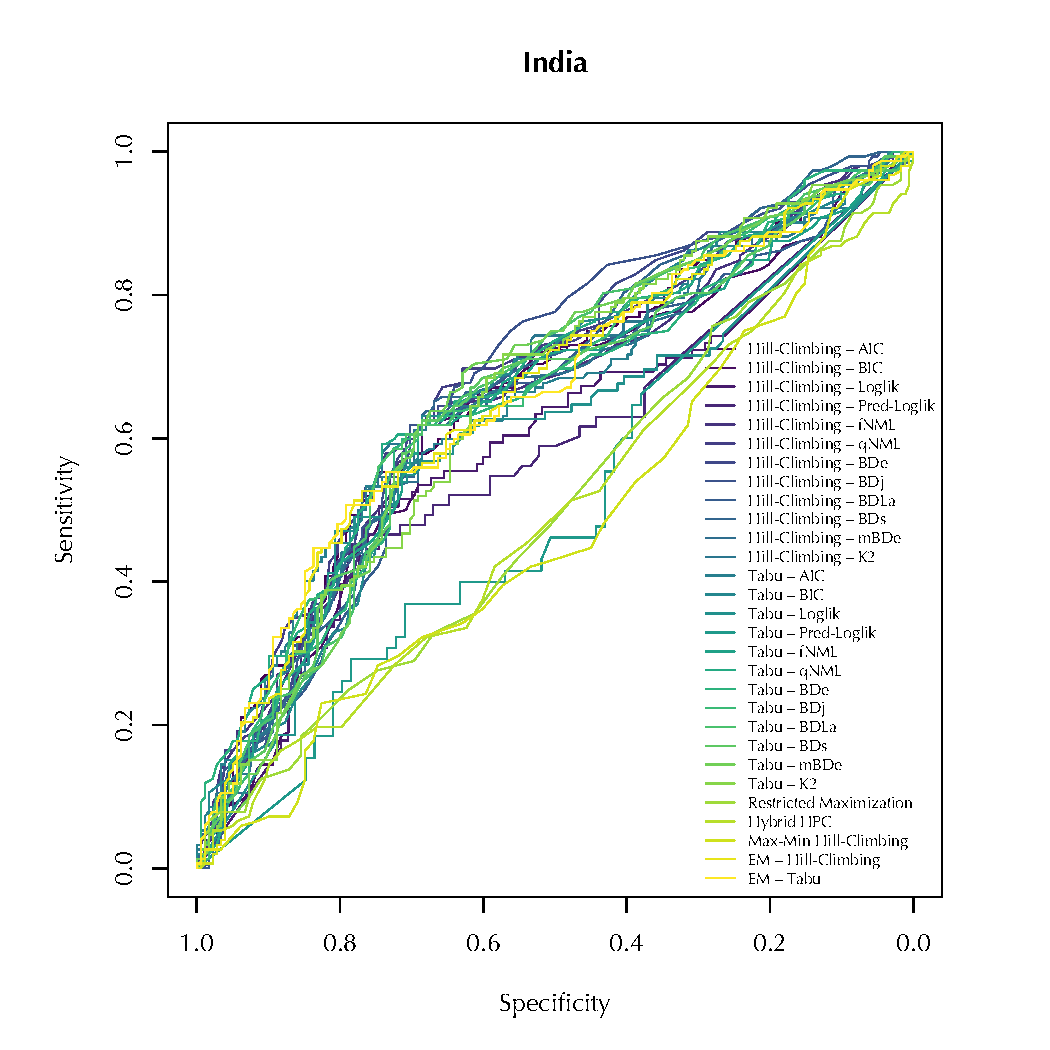
\includegraphics[width=45mm]{../3. Code/Implied Volatility/Exports/ROC/India} &   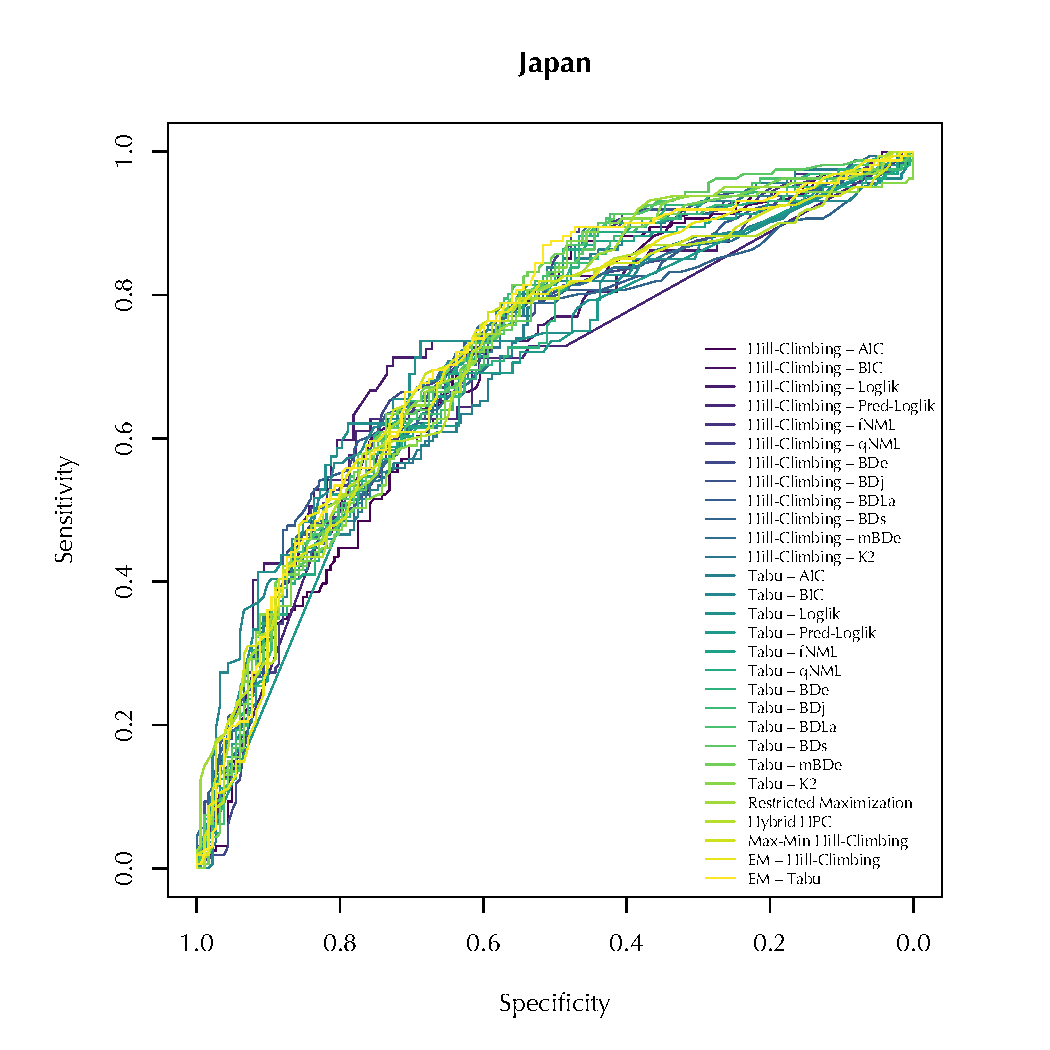
\includegraphics[width=45mm]{../3. Code/Implied Volatility/Exports/ROC/Japan} &    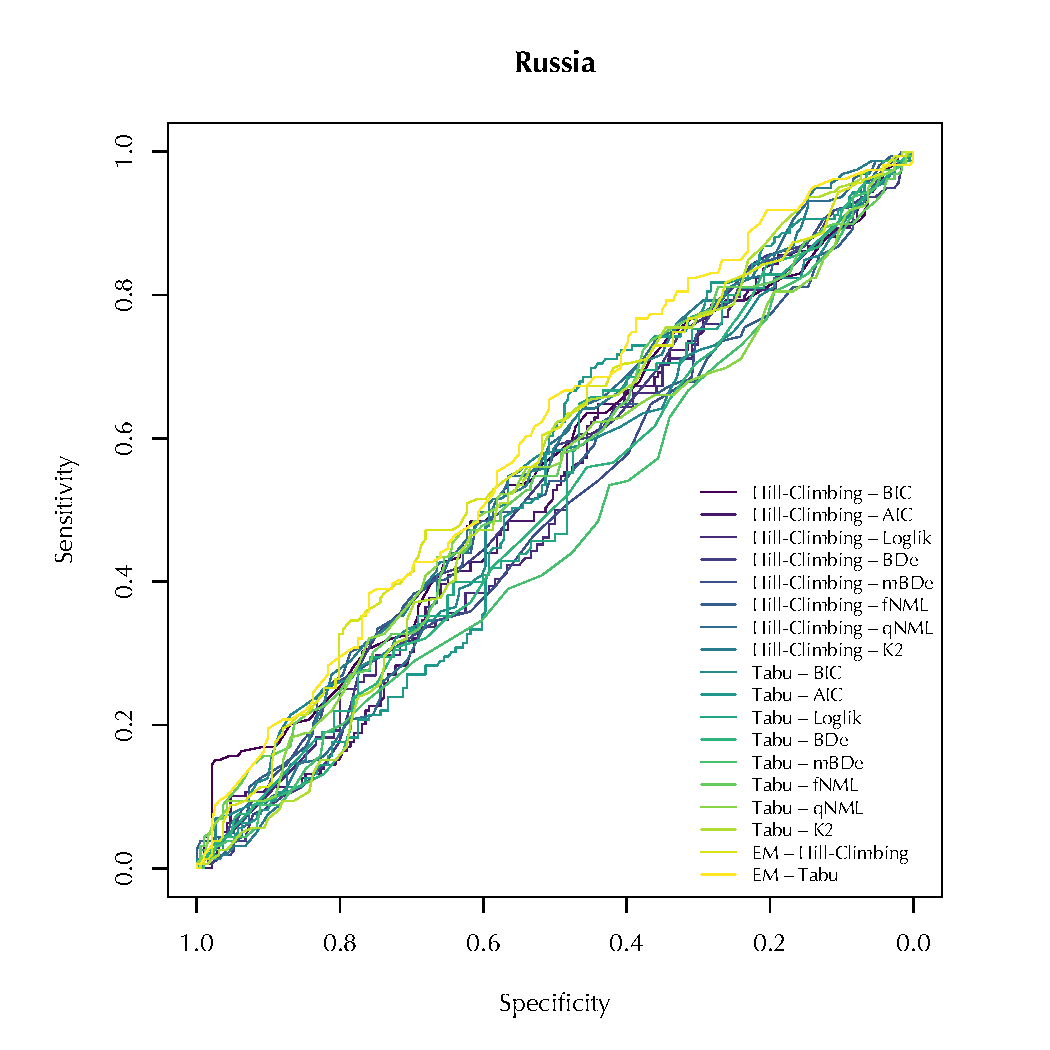
\includegraphics[width=45mm]{../3. Code/Implied Volatility/Exports/ROC/Russia} \\
    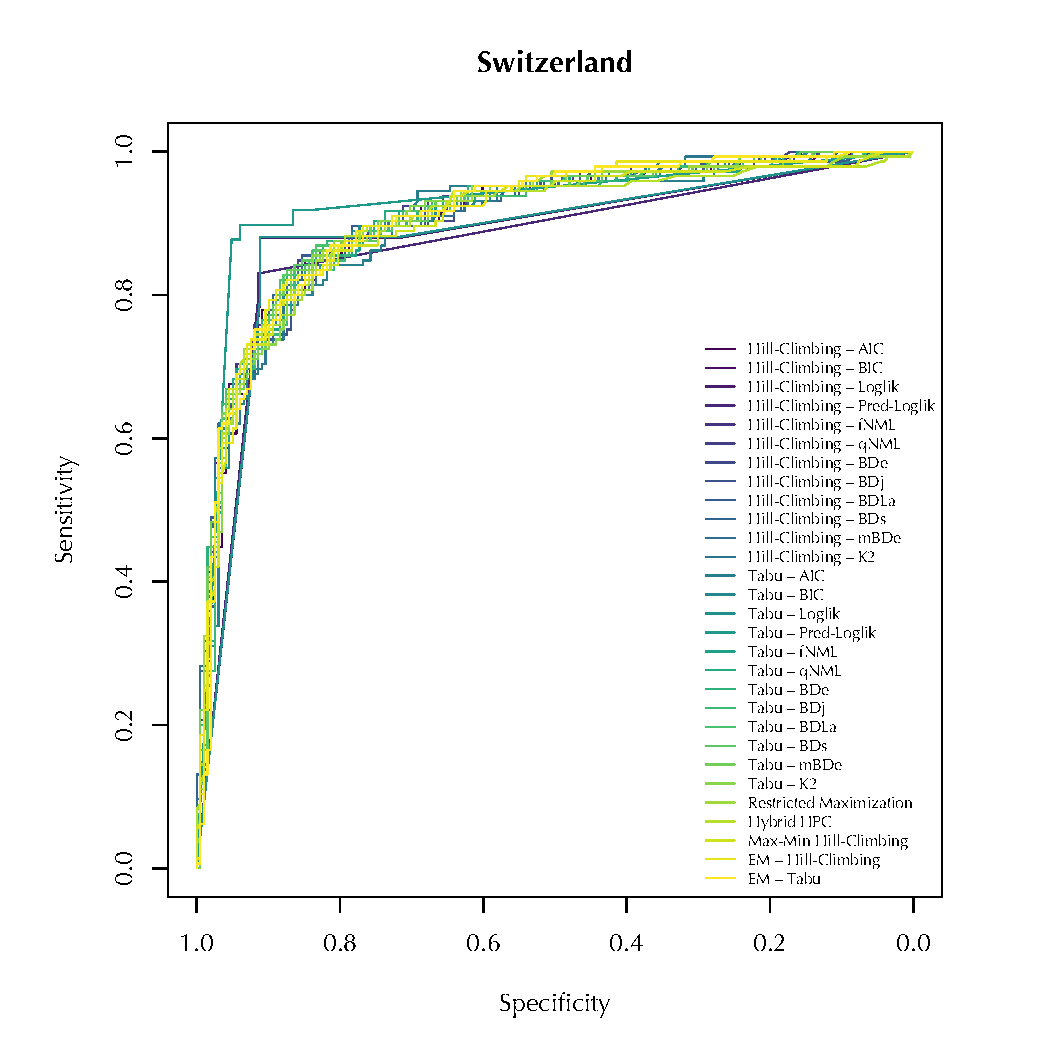
\includegraphics[width=45mm]{../3. Code/Implied Volatility/Exports/ROC/Switzerland} &       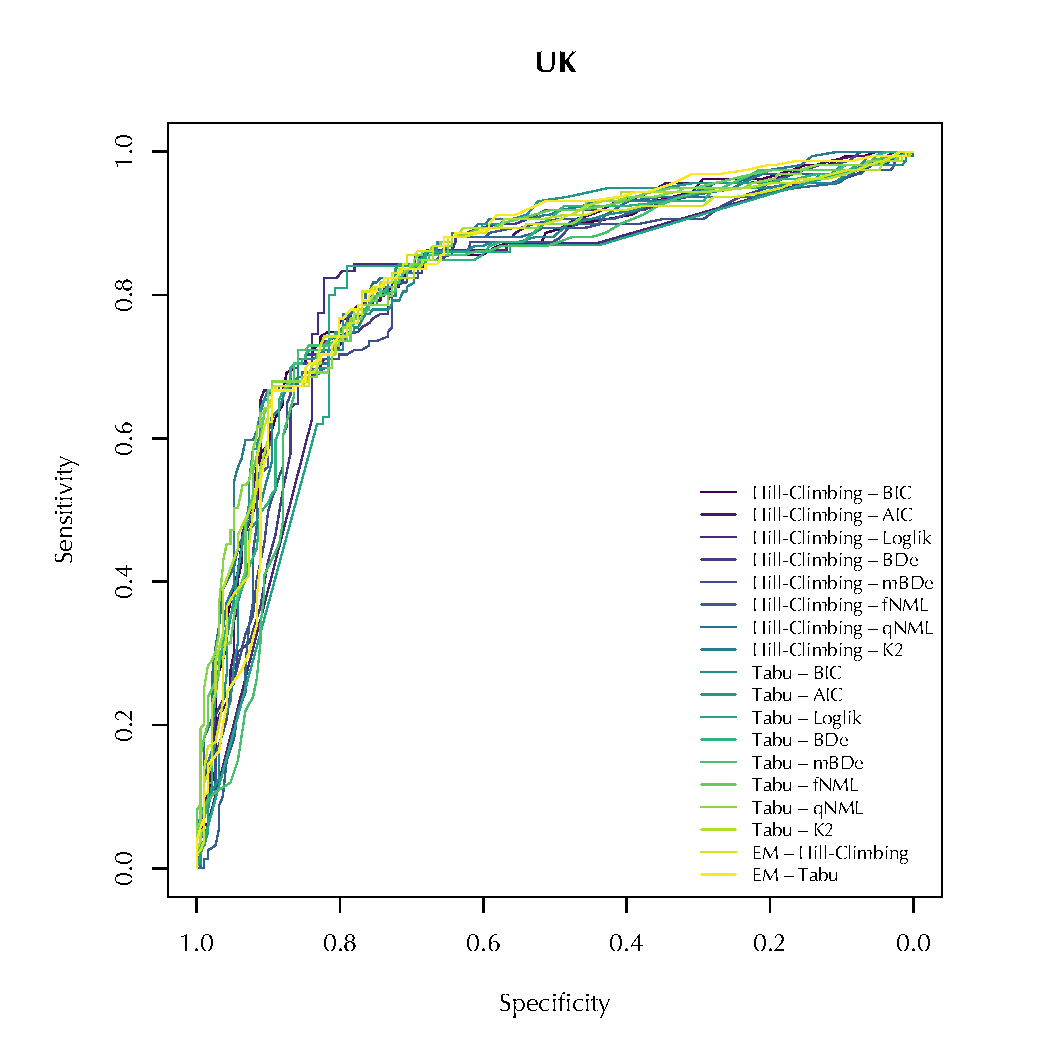
\includegraphics[width=45mm]{../3. Code/Implied Volatility/Exports/ROC/UK} &  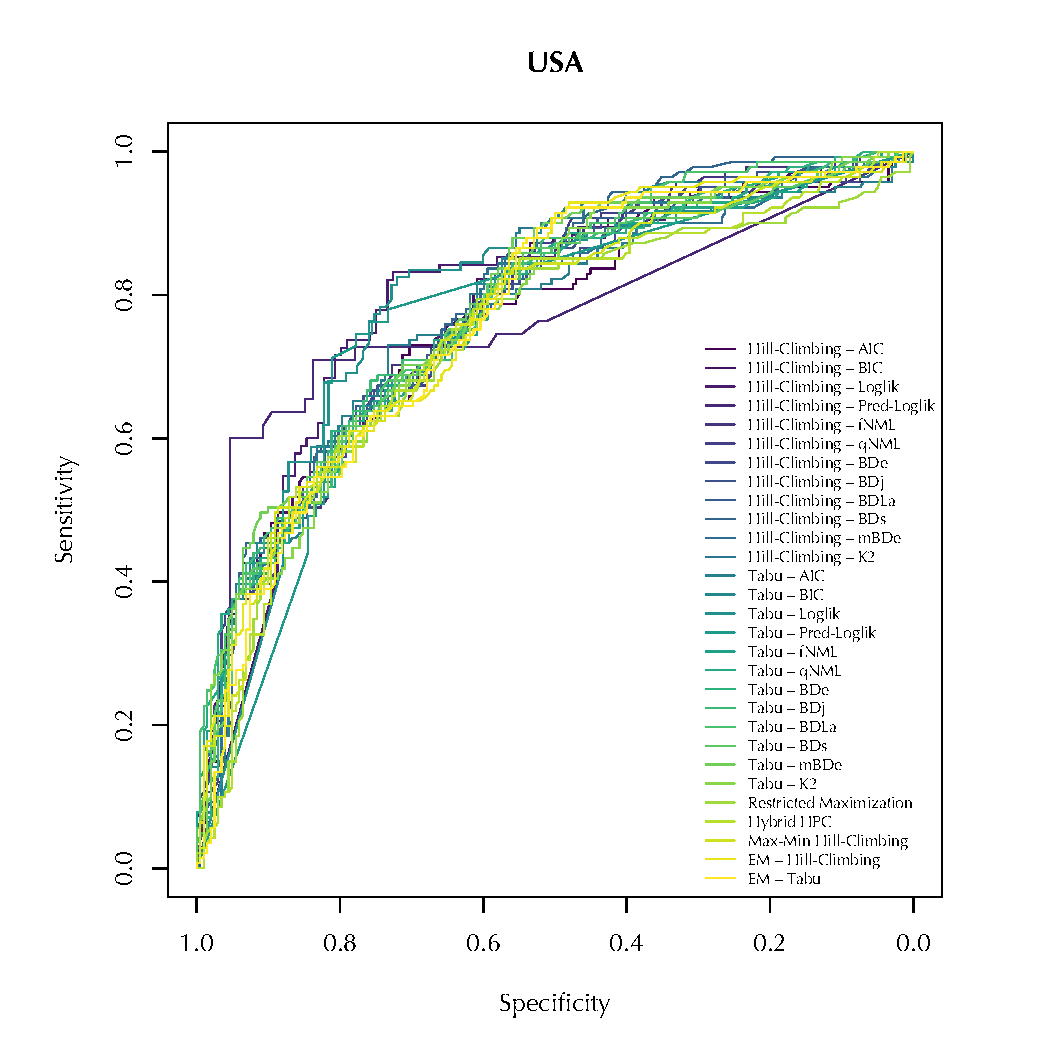
\includegraphics[width=45mm]{../3. Code/Implied Volatility/Exports/ROC/USA}  \\
%(c) third & (d) fourth \\[6pt]
\end{tabular}
\caption[ROC curves of all implemented algorithms per country (node)]{ROC curves of all implemented algorithms per  country (node)}
  \label{fig:roccurves}
\end{figure*}



\section{Evaluating Networks from Implied Volatility Data}
\label{subsec:roc}
To validate our learned Bayesian networks we exploit the binary representation of our data. We make predictions from our networks using \texttt{predict()} and compare them with our test data. \newline \textit{Sensitivity} or true positive rate ($\mathrm{TPR}$) is derived from the true positives $\mathrm{TP}$,  i.e., the correctly identified positives $\mathrm{P}$ from our test set: 
$
\mathrm{TPR}=\frac{\mathrm{TP}}{\mathrm{P}}
$
\newline \textit{Specificity} or true negative rate ($\mathrm{TNR}$) is derived from the true negatives $\mathrm{TN}$,  i.e., the correctly identified negatives $\mathrm{N}$ from our test set: 
$
\mathrm{TNR}=\frac{\mathrm{TN}}{\mathrm{N}}
$
\newline By plotting both the sensitivity and specificity in relation, we obtain the so called Receiver Operating Curve (ROC), where for both measures, 1 or 100\% is the optimum, and if the curve is the diagonal, we observed a random process.  In Figure~\ref{fig:roccurves}, we can see the ROC for each country -- or node in our network in this case -- depicted for each algorithm for comparability. To further summarise these evaluations, we can calculate the Area Under the Curve (AUC) and populate Table~\ref{tab:rocdata} (Appendix),  ordered by the sum of all values to rank our models. Again, a value of 0.5 indicates a random process.  \cite{Hastie2009} \cite{Ertel2020}  \cite{Kauermann2021}  \cite{Russell2021}



As illustrated in Figure~\ref{fig:roccurves} and Table~\ref{tab:rocdata} (Appendix), most countries demonstrated significant predictive qualities. But \textsl{Canada}, \textsl{India}, and especially \textsl{Russia} are very close to a random process. We continue our analysis but consider the possibility of dropping them from our data set and therefore Bayesian networks. \\

We proceed by comparing the best performing networks (in terms of probability distributions) and illustrating their overlap, as shown in Figure~\ref{fig:networkcomparison}.


\begin{figure*}
   \scalebox{0.87}{
\begin{tabular}{cc} 
  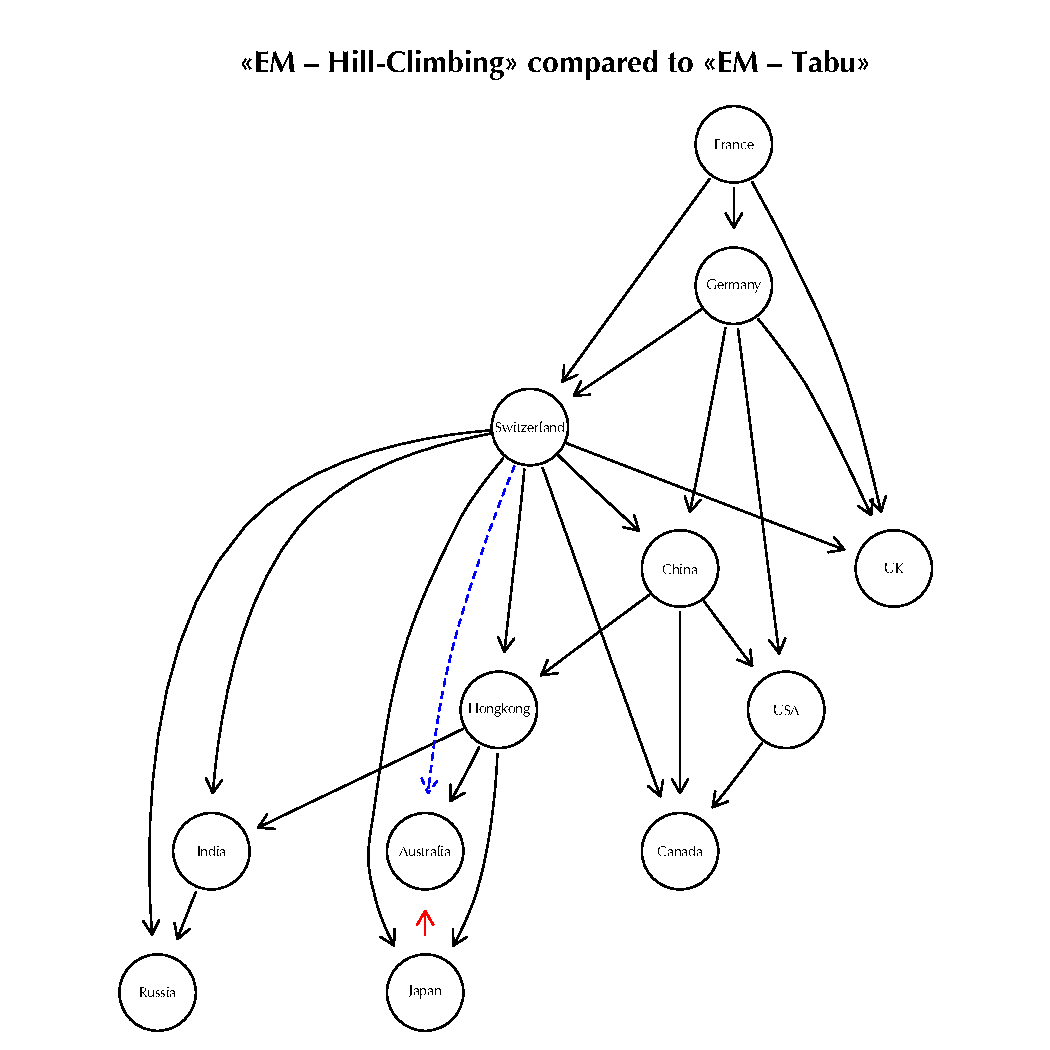
\includegraphics[trim={1.5cm 0 1.5cm 0},clip,width=45mm]{../3. Code/Implied Volatility/Exports/Networks/Comparison1} &   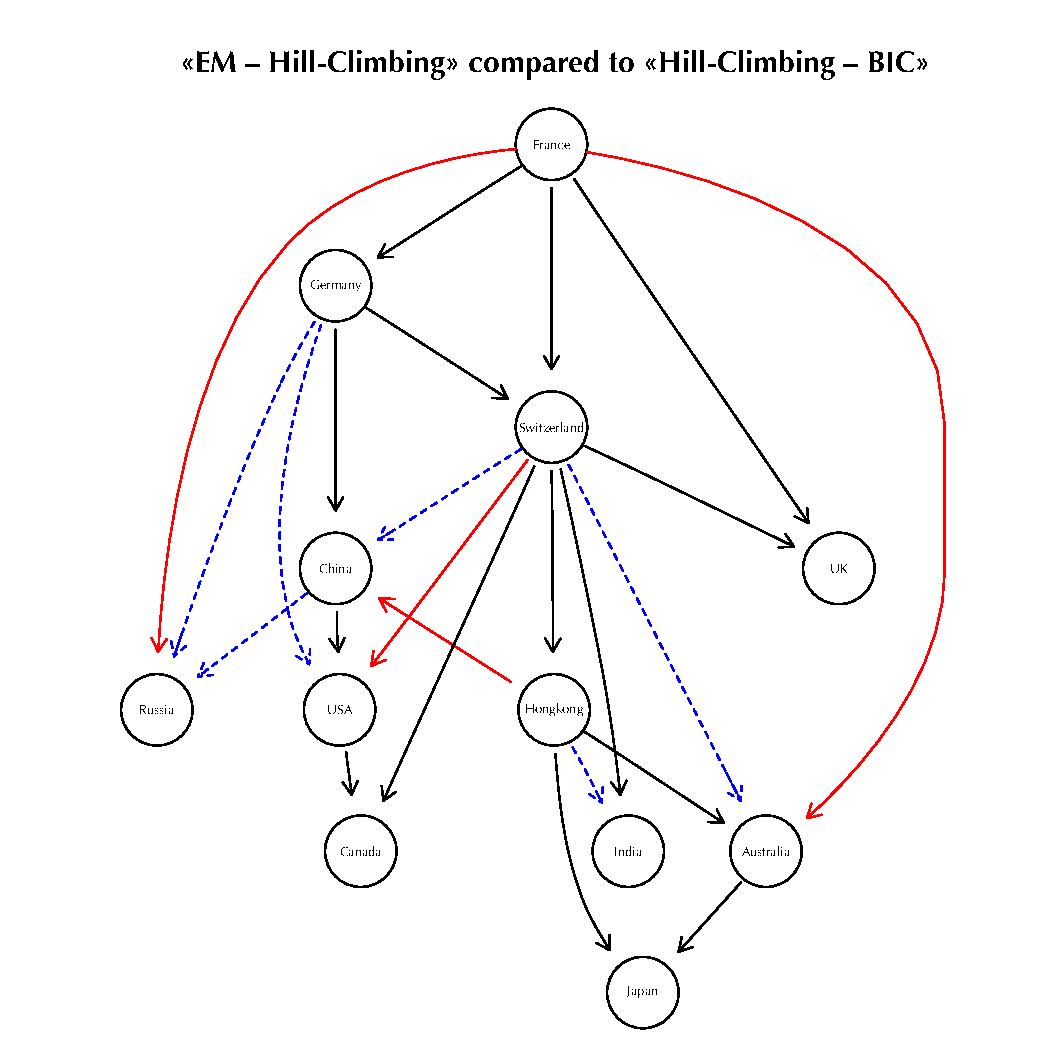
\includegraphics[trim={1.5cm 0 1.5cm 0},clip,width=45mm]{../3. Code/Implied Volatility/Exports/Networks/Comparison2}\\
 \\
  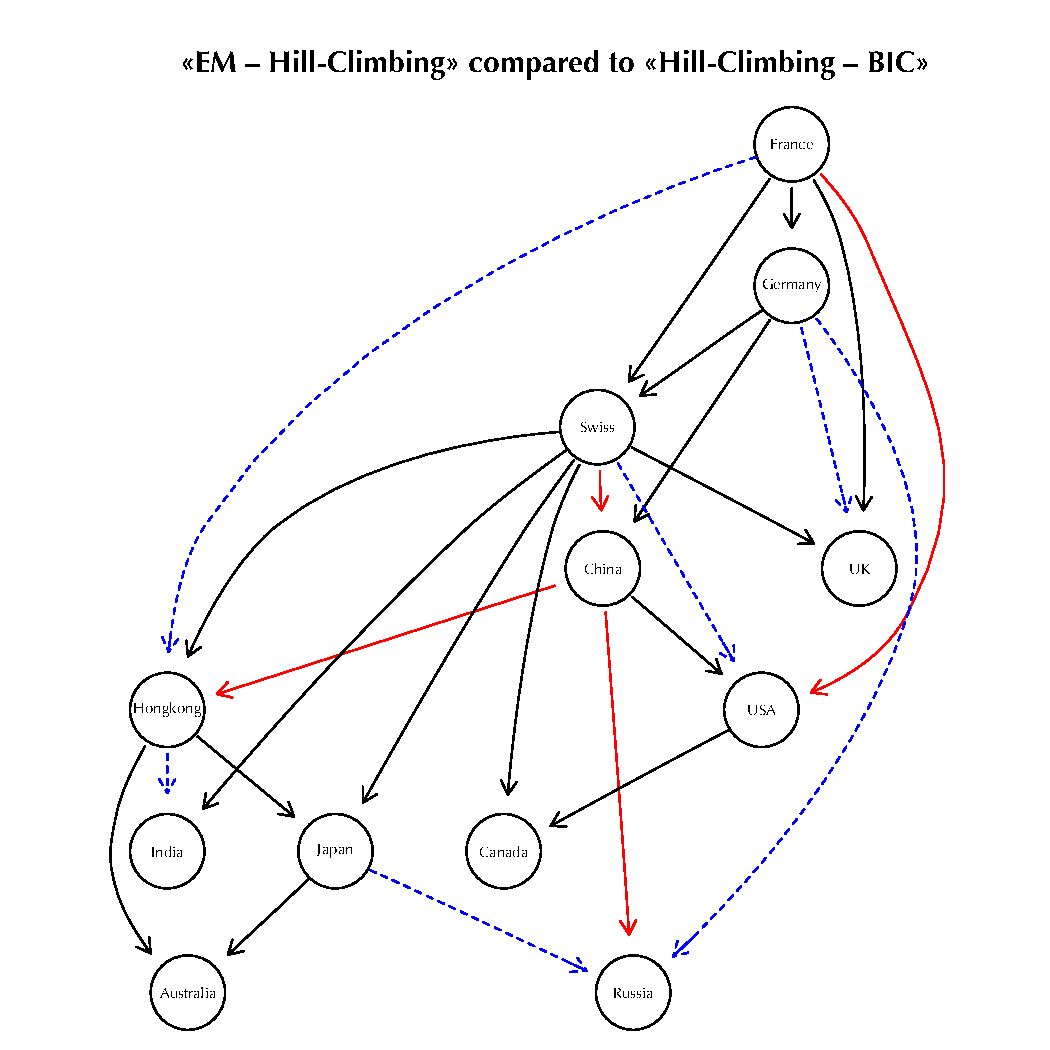
\includegraphics[trim={1.5cm 0 1.5cm 0},clip,width=45mm]{../3. Code/Implied Volatility/Exports/Networks/Comparison3} &   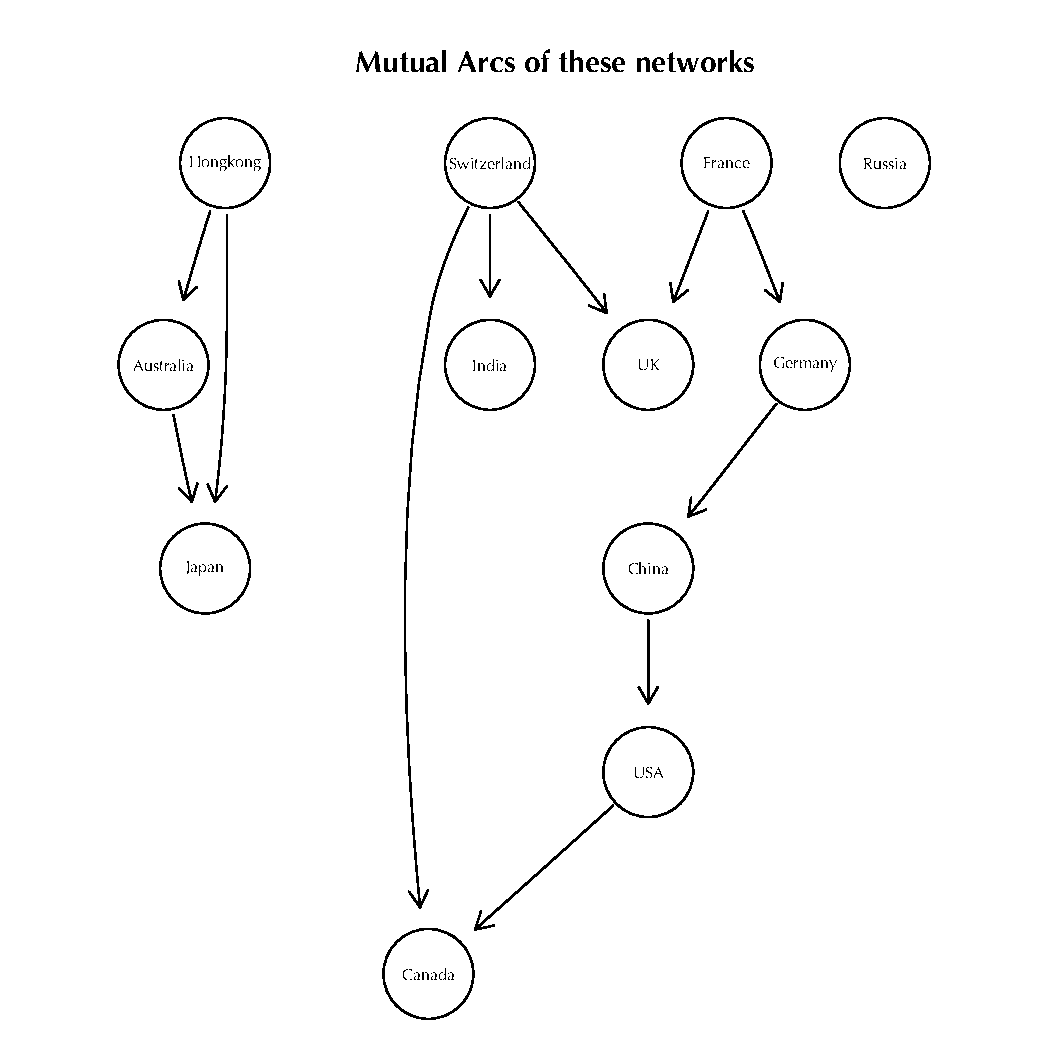
\includegraphics[trim={1.5cm 0 1.5cm 0},clip,width=45mm]{../3. Code/Implied Volatility/Exports/Networks/Comparison4}\\
\end{tabular}
}
\caption[Comparison of networks with highest AUC scores]{Comparison of the three networks with the highest combined AUC scores}
  \label{fig:networkcomparison}
\end{figure*}


After comparing the Bayesian networks in terms of structural similarities, we now examine the reliability of the predictions and the corresponding conditional probabilities. In Figure~\ref{fig:networkcomparison2}, we illustrate this confidence using arc strength and can show that we can expect reliable distributions for \textsl{France}, \textsl{Germany}, and  \textsl{Switzerland} in particular. Table~\ref{tab:cpt} provides an excerpt of some recognisable conditional probabilities.
\begin{figure*}
   \scalebox{0.87}{
%\begin{tabular}{c|c|c}
\begin{tabular}{ccc}
 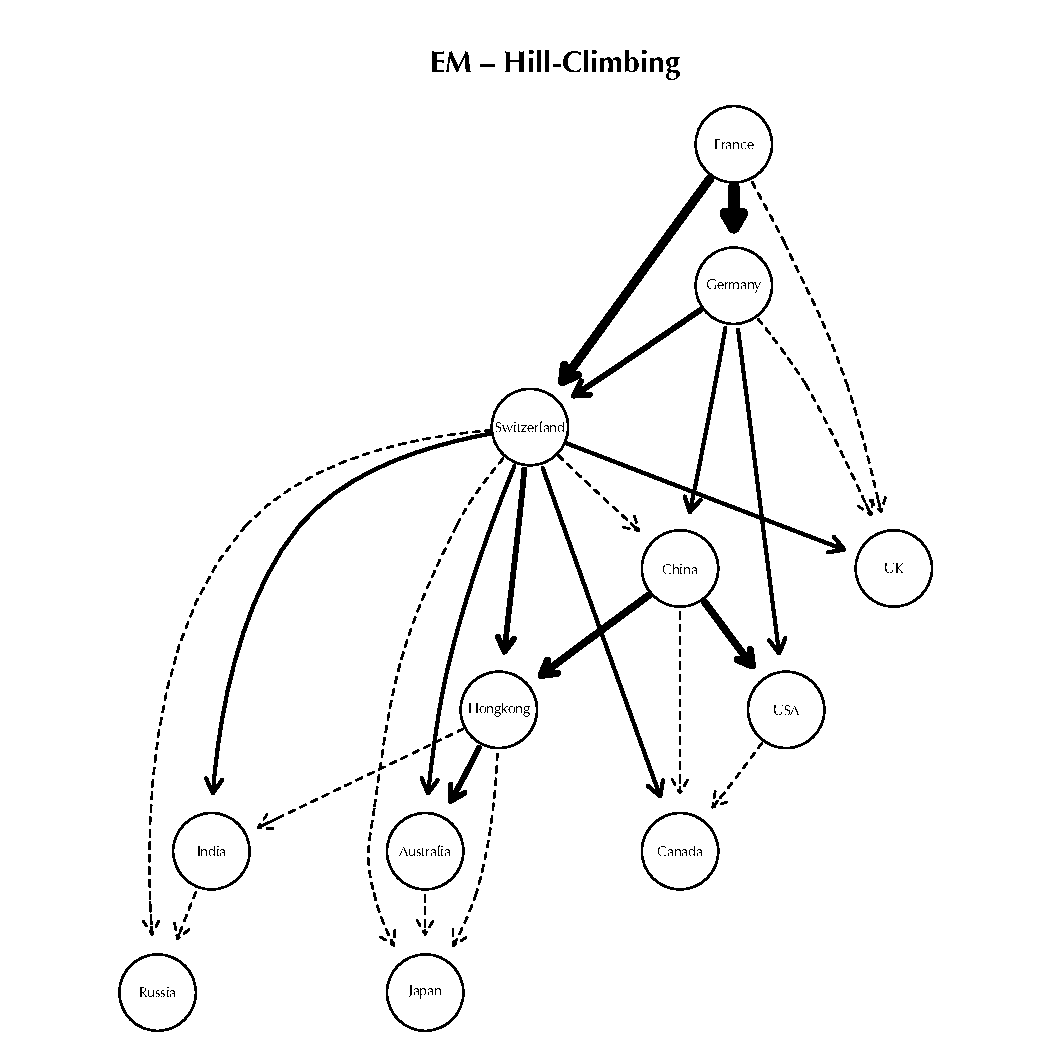
\includegraphics[trim={ 1.5cm  0 1.5cm 0 },clip, width=45mm]{../3. Code/Implied Volatility/Exports/Networks/Strength1} &  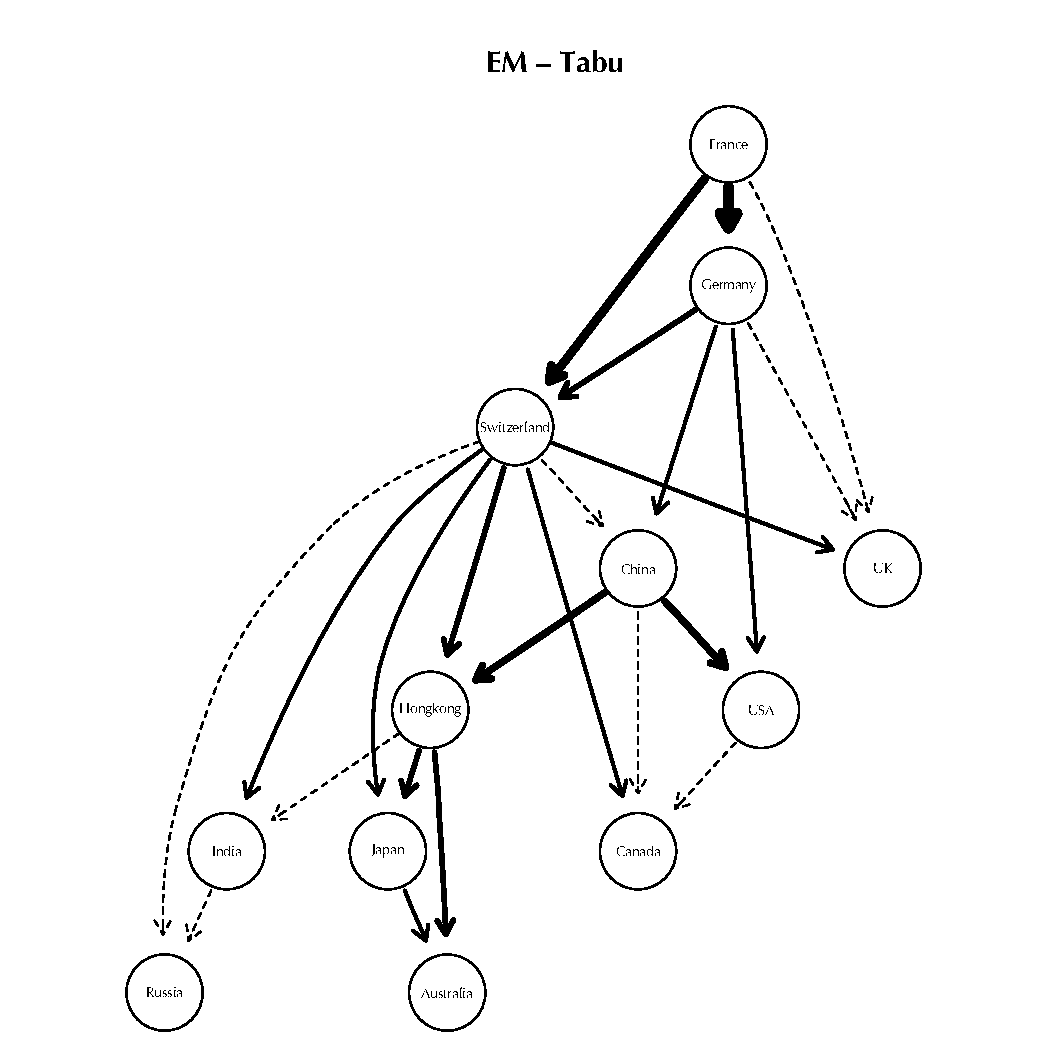
\includegraphics[trim={ 1.5cm  0 1.5cm 0 },clip, width=45mm]{../3. Code/Implied Volatility/Exports/Networks/Strength2}  &  \includegraphics[trim={ 1.5cm  0 1.5cm 0 },clip, width=45mm]{../3. Code/Implied Volatility/Exports/Networks/Strength3}\\
   \includegraphics[trim={ 0 0 0 1.75cm },clip, width=40mm]{../3. Code/Implied Volatility/Exports/ROC/ROC1} &\includegraphics[trim={ 0 0 0 1.75cm },clip, width=40mm]{../3. Code/Implied Volatility/Exports/ROC/ROC2}  &   \includegraphics[trim={ 0 0 0 1.75cm },clip, width=40mm]{../3. Code/Implied Volatility/Exports/ROC/ROC3}    \\
 \end{tabular}
}
\caption[Comparison of the impact of the networks with  highest AUC scores]{Comparison of the three networks with the highest total AUC scores -- confidence depicted as arc strength by $\Delta$ BIC scores.}
  \label{fig:networkcomparison2}
\end{figure*}

\newpage
\clearpage
\section{Causal networks and final result}
\label{subsec:causal}

\vspace*{6mm}

\chapquote{``I would rather discover one causal law  than be King of Persia."}{Dēmókritos}{(460 -- 370 B.C.) \cite[p. 41]{Pearl2009}}

\vspace*{8mm}
When we introduced this use case, we talked about the impact of the countries on each other. But up to this point, we have merely identified significant conditional probabilities -- in other words, correlation, not causation. That is, why we now introduce and apply methods of causal discovery to infer the actual cause -- the desired impact. \cite{Pearl2009}  \cite{Chicharro2014} 

\begin{figure}[H]
\begin{tabular}{cccc}

\begin{subfigure}{.19\linewidth}
  \centering
\begin{tikzpicture}[
  node distance=0.35cm and 0cm,
  mynode/.style={draw,circle,text width=0.15cm, align=center, fill=white, draw=Green, text = Green},
  mycenter/.style={draw,circle,text width=0.15cm,align=center, fill=gray!30}
]
% nodes
%\node[mycenter] (n) {n}; %
 \node[mynode] (a) {\tiny{a}}; %
 \node[mynode,below=of a] (b) {\tiny{b}}; %
 \node[mynode,below=of b] (c) {\tiny{c}}; %
% edges
 \draw[-{Latex[length=1.5mm, width=1mm]}, Green] (b) -- (c);
 \draw[-{Latex[length=1.5mm, width=1mm]}, Green] (a) -- (b);
 \end{tikzpicture}
 \end{subfigure}
 &
 \begin{subfigure}{.19\linewidth}
  \centering
\begin{tikzpicture}[
  node distance=0.35cm and 0cm,
  mynode/.style={draw,circle,text width=0.15cm,align=center, fill=white, draw=Green, text = Green},
  mycenter/.style={draw,circle,text width=0.15cm,align=center, fill=gray!30}
  ]
% nodes
%\node[mycenter] (n) {n}; %
 \node[mynode] (a) {\tiny{a}}; %
 \node[mynode,below=of a] (b) {\tiny{b}}; %
 \node[mynode,below=of b] (c) {\tiny{c}}; %
% edges
 \draw[-{Latex[length=1.5mm, width=1mm]},Green] (c) -- (b);
  \draw[-{Latex[length=1.5mm, width=1mm]},Green] (b) -- (a);
 \end{tikzpicture}
 \end{subfigure}
 &
 \begin{subfigure}{.19\linewidth}
  \centering
\begin{tikzpicture}[
  node distance=0.35cm and 0cm,
  mynode/.style={draw,circle,text width=0.15cm,align=center, fill=white, draw=Green, text = Green},
  mycenter/.style={draw,circle,text width=0.15cm,align=center, fill=gray!30}
  ]
% nodes
%\node[mycenter] (n) {n}; %
 \node[mynode] (a) {\tiny{a}}; %
 \node[mynode,below=of a] (b) {\tiny{b}}; %
 \node[mynode,below=of b] (c) {\tiny{c}}; %
% edges
 \draw[-{Latex[length=1.5mm, width=1mm]}, Green] (b) -- (c);
  \draw[-{Latex[length=1.5mm, width=1mm]}, Green] (b) -- (a);
 \end{tikzpicture}
 \end{subfigure}
 &
 \begin{subfigure}{.19\linewidth}
  \centering
\begin{tikzpicture}[
  node distance=0.35cm and 0cm,
  mynode/.style={draw,circle,text width=0.15cm,align=center, fill=white, draw=red, text = red},
  mycenter/.style={draw,circle,text width=0.15cm,align=center, fill=gray!30}
  ]
% nodes
%\node[mycenter] (n) {n}; %
 \node[mynode] (a) {\tiny{a}}; %
 \node[mynode,below=of a] (b) {\tiny{b}}; %
 \node[mynode,below=of b] (c) {\tiny{c}}; %
% edges
 \draw[-{Latex[length=1.5mm, width=1mm]}, red] (c) -- (b);
  \draw[-{Latex[length=1.5mm, width=1mm]}, red] (a) -- (b);
 \end{tikzpicture}
 \end{subfigure}
 \end{tabular}
 \caption[Markov Equivalence classes]{\small Markov Equivalence}
   \label{fig:markovclass}
\end{figure}
We do not attempt to identify the best causal Bayesian network, but rather a small set of plausible causal Bayesian networks that fit our data.  And there are several methods to learn a causal model directly, but we aim for a more comparable approach (here ROC in Section~\ref{subsec:roc}) and thus derive causality from our networks by causal structure search. \cite{Glymour2019}  For our further approach, it is important to be aware of the Markov equivalence classes: identical adjacencies -- derived from the Markov condition --  and the same \textit{unshielded colliders}. Exemplified for three nodes in Figure~\ref{fig:markovclass} in green. The two cascading arrangements and the pattern of a common parent are all equivalent -- only the v-structure, the unshielded collider, in red does not belong to the equivalence class. Most causal discovery approaches  learn exclusively these equivalence classes. \cite{Pearl2009}  
We broaden our assumptions and in addition to acyclicity we define the following: \cite{Pearl2009}  \cite{Pearl1991} \cite{Spirtes1991}  \cite{Druzdzel2009} \change{include d-separation and explain necessity}
\begin{enumerate}[label=\Roman*]
\item \textit{Causal Markov} assumption -- an extension to our previous Markov assumption: instead of conditional probabilities, a deterministic relationship is implied and nodes are conditionally independent of its non-descendants, given its direct causes.
\item \textit{Causal faithfulness} or stability assumption -- as it assumes all independencies to be stable and thus for any change in the parameters they will remain.
\item \textit{Causal sufficiency} assumption -- of no common confounders: all the common causes of our variables are already present in our network.
\end{enumerate}  
Our causal structure search is based on the \textit{Inductive Causation} algorithm from \textsc{Pearl} and  \textsc{Meek}. The gist is the inductive reasoning of Ockham's razor  to discard any model for which we find a more compact \textit{minimal} model that represents our data equally. This \textit{inferred causation} means in essence, that $a$ is supposed to to have a causal influence on $b$ if there is $a \rightarrow b$  \enquote{in every minimal structure consistent with the data}\cite[p. 45]{Pearl2009}. Thus, the topology of our Bayesian network -- the underlying DAG -- is sufficient for our causal structure search. \cite{Meek1995} \cite{Pearl1991} \cite{Pearl2009} \cite{Druzdzel2009}\\
% Given  the Data  a  variable C  has a causal influence on  E iff there exists a directed path  $C \rightarrow^{*} E $ in every minimal latent  structure consistent with the data
As we learn a causal Markov equivalence class, only unshielded colliders present in our underlying Bayesian network are to be adapted. Any further v-structures  must be avoided, as illustrated in Figure~\ref{fig:causalrules}.  These rules are sound, as any other orientation in these patterns lead to further unshielded colliders or acyclicity. This approach is illustrated as pseudo code in Figure~\ref{fig:causalalgorithm} and implemented in \texttt{R} (Appendix). \cite{Meek1995} \cite{Pearl1991}   

\begin{figure}[H]
   \scalebox{0.5}{
%\begin{tabular}{m{1cm} m{6cm} m{2cm} m{4cm}}
\begin{tabular}{>{\centering\arraybackslash}m{.2\linewidth}>{\centering\arraybackslash}m{.65\linewidth}>{\centering\arraybackslash}m{.2\linewidth}>{\centering\arraybackslash}m{.65\linewidth}}
\textbf{Colliders} &\begin{tikzpicture}[
  node distance=1cm and 0cm,
  mynode/.style={draw,circle,text width=0.7cm,align=center, fill=white},
  mycenter/.style={draw,circle,text width=0.7cm,align=center, fill=gray!30}
]
% nodes
 \node[mycenter] (n) {n}; %
  \node[mynode,left=of n,xshift=-1cm] (a) {a}; %
 \node[mynode,right=of n,xshift=1cm] (b) {b}; %
% edges
  \draw[dashed, -{Latex}] (a) -- (n);
  \draw[dashed, -{Latex}] (b) -- (n);
\end{tikzpicture}
 &$\Longrightarrow$&\begin{tikzpicture}[
  node distance=1cm and 0cm,
  mynode/.style={draw,circle,text width=0.7cm,align=center, fill=white},
  mycenter/.style={draw,circle,text width=0.7cm,align=center, fill=gray!30}
]
% nodes
 \node[mycenter] (n) {n}; %
  \node[mynode,left=of n,xshift=-1cm] (a) {a}; %
 \node[mynode,right=of n,xshift=1cm] (b) {b}; %
% edges
 \draw[-{Latex}] (a) -- (n);
 \draw[-{Latex}] (b) -- (n);
\end{tikzpicture}
 \\
 &&&\\
\textbf{Rule 1} &\begin{tikzpicture}[
  node distance=1cm and 0cm,
  mynode/.style={draw,circle,text width=0.7cm,align=center, fill=white},
  mycenter/.style={draw,circle,text width=0.7cm,align=center, fill=gray!30}
]
% nodes
 \node[mycenter] (n) {n}; %
  \node[mynode,left=of n,xshift=-1cm] (a) {a}; %
 \node[mynode,right=of n,xshift=1cm] (b) {b}; %
% edges
 \draw[-{Latex}] (a) -- (n);
 \draw    (n) -- (b);
\end{tikzpicture}
 &$\Longrightarrow$&\begin{tikzpicture}[
  node distance=1cm and 0cm,
  mynode/.style={draw,circle,text width=0.7cm,align=center, fill=white},
  mycenter/.style={draw,circle,text width=0.7cm,align=center, fill=gray!30}
]
% nodes
 \node[mycenter] (n) {n}; %
  \node[mynode,left=of n,xshift=-1cm] (a) {a}; %
 \node[mynode,right=of n,xshift=1cm] (b) {b}; %
% edges
 \draw[-{Latex}] (a) -- (n);
 \draw[-{Latex}] (n) -- (b);
\end{tikzpicture}
 \\
 &&&\\
 \textbf{Rule 2} &\begin{tikzpicture}[
  node distance=1cm and 0cm,
  mynode/.style={draw,circle,text width=0.7cm,align=center, fill=white},
  mycenter/.style={draw,circle,text width=0.7cm,align=center, fill=gray!30}
]
% nodes
 \node[mycenter] (n) {n}; %
  \node[mynode,below=of n,xshift=-1.5cm] (a) {a}; %
 \node[mynode,below=of n,xshift=1.5cm] (b) {b}; %
% edges
 \draw[-{Latex}] (n) -- (a);
 \draw[-{Latex}] (a) -- (b);
 \draw    (n) -- (b);
\end{tikzpicture}
 & $\Longrightarrow$&\begin{tikzpicture}[
  node distance=1cm and 0cm,
  mynode/.style={draw,circle,text width=0.7cm,align=center, fill=white},
  mycenter/.style={draw,circle,text width=0.7cm,align=center, fill=gray!30}
]
% nodes
\node[mycenter] (n) {n}; %
  \node[mynode,below=of n,xshift=-1.5cm] (a) {a}; %
 \node[mynode,below=of n,xshift=1.5cm] (b) {b}; %
% edges
 \draw[-{Latex}] (n) -- (a);
 \draw[-{Latex}] (a) -- (b);
 \draw[-{Latex}] (n) -- (b);
 \end{tikzpicture}\\
 &&&\\
 \textbf{Rule 3} &\begin{tikzpicture}[
  node distance=1cm and 0cm,
  mynode/.style={draw,circle,text width=0.7cm,align=center, fill=white},
  mycenter/.style={draw,circle,text width=0.7cm,align=center, fill=gray!30}
]
% nodes
\node[mycenter] (n) {n}; %
  \node[mynode,below=of n,xshift=-1.5cm] (a) {a}; %
 \node[mynode,below=of n,xshift=1.5cm] (c) {c}; %
  \node[mynode,below=of a,xshift=1.5cm] (b) {b}; %
% edges
 \draw[-{Latex}] (c) -- (b);
 \draw[-{Latex}] (a) -- (b);
    \draw    (n) -- (a);
 \draw    (n) -- (b);
  \draw    (n) -- (c);
\end{tikzpicture}
 & $\Longrightarrow$&\begin{tikzpicture}[
  node distance=1cm and 0cm,
  mynode/.style={draw,circle,text width=0.7cm,align=center, fill=white},
  mycenter/.style={draw,circle,text width=0.7cm,align=center, fill=gray!30}
]
% nodes
\node[mycenter] (n) {n}; %
  \node[mynode,below=of n,xshift=-1.5cm] (a) {a}; %
 \node[mynode,below=of n,xshift=1.5cm] (c) {c}; %
  \node[mynode,below=of a,xshift=1.5cm] (b) {b}; %
% edges
 \draw[-{Latex}] (c) -- (b);
 \draw[-{Latex}] (a) -- (b);
    \draw    (n) -- (a);
 \draw[-{Latex}] (n) -- (b);
  \draw    (n) -- (c);
 \end{tikzpicture}\\
  &&&\\
 \textbf{Rule 4} &\begin{tikzpicture}[
  node distance=1cm and 0cm,
  mynode/.style={draw,circle,text width=0.7cm,align=center, fill=white},
  mycenter/.style={draw,circle,text width=0.7cm,align=center, fill=gray!30}
]
% nodes
\node[mycenter] (n) {n}; %
  \node[mynode,below=of n,xshift=-1.5cm] (a) {a}; %
 \node[mynode,below=of n,xshift=1.5cm] (c) {c}; %
  \node[mynode,below=of a,xshift=1.5cm] (b) {b}; %
% edges
 \draw[-{Latex}] (b) -- (c);
 \draw[-{Latex}] (a) -- (b);
    \draw    (n) -- (a);
 \draw    (n) -- (b);
  \draw    (n) -- (c);
\end{tikzpicture}
 & $\Longrightarrow$&\begin{tikzpicture}[
  node distance=1cm and 0cm,
  mynode/.style={draw,circle,text width=0.7cm,align=center, fill=white},
  mycenter/.style={draw,circle,text width=0.7cm,align=center, fill=gray!30}
]
% nodes
\node[mycenter] (n) {n}; %
  \node[mynode,below=of n,xshift=-1.5cm] (a) {a}; %
 \node[mynode,below=of n,xshift=1.5cm] (c) {c}; %
  \node[mynode,below=of a,xshift=1.5cm] (b) {b}; %
% edges
 \draw[-{Latex}] (b) -- (c);
 \draw[-{Latex}] (a) -- (b);
    \draw    (n) -- (a);
 \draw[-{Latex}] (n) -- (c);
    \draw    (n) -- (b);
 \end{tikzpicture}\\
 \end{tabular}
}
\caption[Rules of orientation]{After orienting the unshielded colliders present in our original Bayesian network once, we follow these four rules of the Inductive Causation algorithm repeatedly until convergence to obtain a maximally oriented Partially Directed Acyclical Graph (PDAG).}
  \label{fig:causalrules}
\end{figure}




Now we can apply our algorithm from Figure~\ref{fig:causalalgorithm} and discuss the results. In Figure~\ref{fig:causalresults1} our two best performing networks could barely be oriented, only the Hill-Climbing – qNML network has significant orientations. But as we are interested in causal networks with both many orientations and good predictive qualities, we expand our focus to the best quantile in terms of AUC. Thus the additional causal networks in Figure~\ref{fig:causalresults1}. Also for Tabu – qNML we can orient most of the edges and only \textsl{India} -- \textsl{Switzerland} and \textsl{UK} -- \textsl{France} is missing a directed arc. Furthermore, as \textsl{Russia} is no part of the network and thus no cause for any effects, we can now remove it from our data set due to its low significance in our ROC analysis. \textsl{Canada} and \textsl{India} will remain in our data set, as their AUC scores are not necessarily random.

\begin{figure}[H]
   \scalebox{0.45}{
\begin{tabular}{cc}
 \includegraphics[trim={ 1.5cm  0 1.5cm 0 },clip, width=75mm]{../3. Code/Implied Volatility/Exports/Networks/Causal/Causal1} &  \includegraphics[trim={ 1.5cm  0 1.5cm 0 },clip, width=75mm]{../3. Code/Implied Volatility/Exports/Networks/Causal/Causal2}\\
 \\
 \\
 \includegraphics[trim={ 1.5cm  0 1.5cm 0 },clip, width=75mm]{../3. Code/Implied Volatility/Exports/Networks/Causal/Causal3}& \includegraphics[trim={ 1.5cm  0 1.5cm 0 },clip, width=75mm]{../3. Code/Implied Volatility/Exports/Networks/Causal/Causal4} \\  
 \\
 \\
 \includegraphics[trim={ 1.5cm  0 1.5cm 0 },clip, width=75mm]{../3. Code/Implied Volatility/Exports/Networks/Causal/Causal5}  &  \includegraphics[trim={ 1.5cm  0 1.5cm 0 },clip, width=75mm]{../3. Code/Implied Volatility/Exports/Networks/Causal/Causal6}\\
 \end{tabular}
}
\caption[Comparison of the impact of the networks with  highest AUC scores]{Comparison of the networks from the highest quantile in terms of AUC scores.}
  \label{fig:causalresults1}
\end{figure}
\newpage
\begin{figure}[H]
\centering
  \includegraphics[trim={0 0 0 0},clip, height=0.72\textwidth]{../3. Code/Implied Volatility/Exports/Networks/Causal/Final Causal}
  \caption[Final causal structure]{Final causal structure: overlap of our networks with the most orientations in the highest quantile of total AUC.}
  \label{fig:finalcausal}
\end{figure}

For the two causal networks with the most orientations, it can be argued that \textsl{Switzerland} is the financial hub. As described in the Appendix, \textsl{China}'s underlying is traded in the USA, but tracks Chinese equities traded on the Hongkong stock exchange. This explains the connection between \textsl{China}, \textsl{USA}, and \textsl{Hongkong}. So without \textsl{China} -- or with more reliable data on China's implied volatility --  \textsl{Switzerland} divides the network into a western and an eastern hemisphere with dedicated sub-clusters. Thus, the time zones and consequently the tradable hours could be an important generating process for the data. 
%For all five of our causal networks, \textsl{Switzerland}'s role is imminent -- even if the outgoing directed arcs could not be learned in all networks, a small thought experiment provides some confidence:   Based on \textsc{Pearl} \cite{Pearl1991} we learn projections of \textit{the}  minimal causal structure, a Markov equivalence class of the same underlying distribution -- meaning all adjacencies and all unshielded colliders are the same. So for every (except one) arc directed to  \textsl{Switzerland}, the network would effectively result in another unshielded collider -- leading to a contradiction. 
%Pearl1991: We learn projections of the minimal causal model --> Equivalence class --> all colliders are the same --> no other orientation (besides one) is possible ->Switzerland is certain Hub
%2 gleiche distributions -> 2 gleiche sets von Nachbarn -> 2 gleiche colliders -> --> Alle bis auf einen orientierbar, da: irgendeine Kante umorientieren -> Netz passt immer noch --> zweite kante orientieren -> Regelbruch durch collider --> einzige logische Schlussfolgerung: Alle Kanten bis auf eine (nicht klar welche) orientierbar aus der Schweiz //May 27 Notebook Notes 
Although we cannot draw many conclusions, \textsl{Switzerland}'s role as a global financial epicenter seems very intuitive.
\newpage
\section{Critique}
Even if impacts can be discovered without chronological temporal information, causal discovery can only benefit from it. Thus, with intraday data this approach would be even more reliable. Also, with respect to \textit{measurement errors}, with more granular data our models would be more resilient, e.g., to the influence of high-frequency traders and other speculators.  Currently, we have to assume that our multivariate time series of ten years is invariant. However, since the underlying generating process changes frequently, this likely results in an under-fit  for our averaged static model.  Thus, \textit{dynamic} Bayesian networks could be implemented with a shorter (but denser) time frame and validated by rolling windows and tested against recent unseen data. \cite{Pearl1991}  \cite{Glymour2019}  \cite{Nagarajan2014} 

Overall, our approach of inferred causation is based on assumptions that are unlikely to apply to our use case and need to be carefully evaluated.  We included only the largest global financial players, no other countries, and most importantly, no other variables. Thus, on the one hand, the \textit{selection bias}  and, on the other hand, the assumption that there are no common confounding factors are very fragile: why should implied volatility not also be influenced by completely different processes? Thus, even if the IC algorithm works with latent variables, we need to include more detailed and comprehensive data from more potential influencers and then implement a dynamic approach. \cite{Borgelt1999} \cite{Glymour2019} \cite{Pearl1991}


\newpage
\null
\newpage
\onecolumn
\section*{Appendix}


\begin{table}[H]
\centering 
  \caption[Comparison of scoring functions]{Overview of all scoring functions available using \textsc{bnlearn} and implemented with Hill-Climbing and Tabu. \cite{Carvalho2009} \cite{Scutari2019b} \cite{Scutari2022}} 
  \label{tab:score} 
   \scalebox{0.85}{
\begin{tabular}{@{\extracolsep{5pt}}lllcc} 
\\[-5.5ex]  \\\hline \\[-2.5ex]  \hline \\[-2ex] 
Abbreviation   &Name  & Category & Score equivalent  \\
\\[-1.8ex]\hline \noalign{\vskip 2mm} 
AIC&Akaike Information Criterion&  Information-theoretic & \cmark \\
BIC &Bayesian Information Criterion  &  Information-theoretic  & \cmark  \\
fNML&factorised Normalized Maximum Likelihood & Information-theoretic  & \xmark \\
qNML&quotient Normalized Maximum Likelihood&  Information-theoretic  &\cmark \\
Loglik&Log-likelihood  & Information-theoretic& \cmark \\ 
Pred-Loglik&Predictive Log-likelihood  & Information-theoretic& \cmark \\ 
BDe&Bayesian Dirichlet equivalent  & Bayesian& \cmark \\
BDj&Bayesian Dirichlet equivalent (Jeffrey's prior) & Bayesian& \xmark \\
BDLa&locally averaged Bayesian Dirichlet  & Bayesian& \xmark \\
BDs&Bayesian Dirichlet sparse  & Bayesian& \xmark \\
mBDe& modified Bayesian Dirichlet equivalent&  Bayesian  & \xmark \\
K2&K2& Bayesian  & \xmark \\
\\[-1.5ex]  \hline \\[-2.5ex]  \hline \\[-2ex] 
\end{tabular} 
}
\end{table} 



\begin{table}[!htbp] 
\centering 
  \caption[Selected conditional probabilities from learned networks]{Excerpt of some recognisable conditional probabilities conducted with \texttt{cpquery}: since the structures are not identical, these values cannot be retrieved directly from the conditional probability tables.}  
\label{tab:cpt} 
  \scalebox{0.88}{
\begin{tabular}{ 
    l % label
    *3{S[
           % scientific-notation = true,
            round-mode = figures,
            round-precision = 2,
           % table-format=1.2e-1
        ]}}
\\[-5.5ex]  \\\hline \\[-2.5ex]  \hline \\[-2ex] 
Conditional Probability		&\text{EM -- Hill-Climbing}& \text{EM -- Tabu} & \text{Hill-Climbing -- qNML}\\
\\[-1.8ex]\hline \noalign{\vskip 2mm} 
$P( \textsl{Germany} \mid \textsl{  France}) $		& 0.832 & 0.833 & 0.860\\
$P( \textsl{Switzerland} \mid \textsl{  France, Germany}) $		& 0.853 & 0.853 & 0.830\\
$P(\neg \textsl{UK} \mid \textsl{  $\neg$France, $\neg$Germany, $\neg$Switzerland}) $		& 0.854 & 0.854 & 0.850\\
$P( \textsl{Hongkong} \mid \textsl{ China, Switzerland}) $ & 0.693 & 0.693 & 0.585\\
$P( \textsl{China} \mid \textsl{ Switzerland, USA})$& 0.742 & 0.741 & 0.677\\
$P( \textsl{USA} \mid \textsl{ China, Germany}) $& 0.686 & 0.685 & 0.658\\
\\[-1.5ex]  \hline \\[-2.5ex]  \hline \\[-2ex] 
\end{tabular} 
}
\end{table} 


\begin{figure}
\begin{algorithm}[H]
\footnotesize
%\algsetup{linenosize=\tiny}
 \begin{algorithmic}[1]
     \caption{Inductive Causation  based on  \textsc{Pearl} and  \textsc{Meek}}
 \Require{Bayesian network (BN) from \texttt{bnlearn}} 
\Ensure{Partially Directed Acyclic Graph (PDAG) in  \texttt{bnlearn}}
\Procedure{Inductive Causation}{$BN$} 
        \State $PDAG \gets $ skeleton($BN$) 
        	\For{nodes $n$ in $PDAG$}
  		\If{ neighbours$(n)>1$ } 
			\For{ permutations $(a, b)$ of neighbours$(n)$} 
				\If{arcs $a  \rightarrow n$ and $b \rightarrow n$ exist in $BN$}
      					\If{no edge between $a, b$ }
            					 	\State add arcs $a  \rightarrow n$ and $b \rightarrow n$  \Comment{C\phantom{1}} 
					\EndIf
				\EndIf
			\EndFor
		\EndIf
	\EndFor
	\State new.arcs = TRUE 
	\While{ new.arcs = TRUE}
		\State new.arcs = FALSE 
		\For{nodes $n$ in $PDAG$}
			\If{ neighbours$(n)>1$ }
			\For{ permutations $(a, b)$ of neighbours$(n)$} 
				\If{no edge between $a, b$ }
					\If{$(a  \rightarrow n)$ and \textbf{not} $(b  \rightarrow n)$}
						\State add arc $n  \rightarrow b$ and new.arcs = TRUE \Comment{R1} 
					\EndIf
				\EndIf
				\If{$b$ in descendants$(n)$ and \textbf{not} $(b  \rightarrow n)$ }
					\State add arc $n  \rightarrow b$ and new.arcs = TRUE  \Comment{R2} 
				\EndIf				
			\EndFor
			\EndIf
			\If{  neighbours$(n)>2$ }
				\For{ permutations $(a, b, c)$ of neighbours$(n)$} 
					\If{$(a \rightarrow b)$ and $(c  \rightarrow b)$}
						\State add arc $n  \rightarrow b$ and new.arcs = TRUE  \Comment{R3} 
					\EndIf
					
					\If{$(a \rightarrow b)$ and $(b \rightarrow c)$}
						\State add arc $n  \rightarrow c$  and new.arcs = TRUE  \Comment{R4} 
					\EndIf
			\EndFor
			\EndIf
		\EndFor		
	\EndWhile
 \EndProcedure
  \end{algorithmic}
\end{algorithm} 
\caption[Inductive Causation algorithm]{The algorithm based on  \textsc{Pearl} and  \textsc{Meek} uses \texttt{bnlearn} methods  ``\texttt{skeleton}'', ``\texttt{neighbours}''  and ``\texttt{descendants}'' and only adds arcs if the PDAG remains acyclical. }
  \label{fig:causalalgorithm}
\end{figure}


\begin{sidewaystable}[!htbp] \centering 
  \caption[Results of AUC -- Area under the ROC curves]{Area under the ROC curves -- ranked highest to lowest}  
  \label{tab:rocdata} 
  \scalebox{0.65}{
  \renewcommand*{\arraystretch}{1.4}
  \begin{tabularx}{1.3\textwidth}{lrrrrrrrrrrrrr}
%\begin{tabularx}{1.2\textwidth}{lllXllX}
\\[-5.5ex]  \\\hline \\[-3.5ex]  \hline \\[-2ex] 
%data source as link with date (volaitility calculation method?)
  Algorithm & \textsl{Australia} & \textsl{Canada} & \textsl{China} & \textsl{France }& \textsl{Germany} & \textsl{Hongkong }& \textsl{India }& \textsl{Japan }& \textsl{Russia }& \textsl{Switzerland }& \textsl{UK} &\textsl{ USA} & $\sum$ \textbf{AUC}\\
\\[-1.8ex]\hline \noalign{\vskip 2mm} 
 EM – Tabu & 0.714457 & 0.710526 & 0.801356 & 0.935114 & 0.935456 & 0.804403 & 0.667599 & 0.748692 & 0.603444 & 0.911532 & 0.838552 & 0.763433 & \textbf{9.434565}\\
EM – HC & 0.715970 & 0.699063 & 0.788222 & 0.932255 & 0.934769 & 0.806075 & 0.659308 & 0.734171 & 0.589861 & 0.912596 & 0.836478 & 0.763318 & \textbf{9.372085}\\
Tabu – BIC & 0.716891 & 0.709326 & 0.780017 & 0.927320 & 0.924025 & 0.785356 & 0.632751 & 0.731162 & 0.571701 & 0.910025 & 0.816523 & 0.737721 & \textbf{9.242818}\\
Tabu – FNML & 0.727862 & 0.710461 & 0.779239 & 0.925556 & 0.935750 & 0.778078 & 0.634877 & 0.737049 & 0.516135 & 0.903620 & 0.839178 & 0.744050 & \textbf{9.231854}\\
Tabu – K2 & 0.732895 & 0.715789 & 0.789562 & 0.924690 & 0.932283 & 0.777406 & 0.613455 & 0.707663 & 0.549853 & 0.905504 & 0.813478 & 0.741924 & \textbf{9.204501}\\
Tabu – QNML & 0.725049 & 0.692155 & 0.782548 & 0.924020 & 0.930256 & 0.785356 & 0.641712 & 0.716706 & 0.522342 & 0.902441 & 0.826567 & 0.750082 & \textbf{9.199233}\\
Hill-Climbing – FNML & 0.732648 & 0.706234 & 0.770505 & 0.925245 & 0.915162 & 0.782209 & 0.638295 & 0.723639 & 0.537456 & 0.902277 & 0.825826 & 0.736996 & \textbf{9.196491}\\
Hill-Climbing – AIC & 0.735428 & 0.718026 & 0.781621 & 0.922157 & 0.928522 & 0.776505 & 0.613798 & 0.719126 & 0.534986 & 0.903063 & 0.830765 & 0.723925 & \textbf{9.187923}\\
Hill-Climbing – QNML & 0.726464 & 0.682451 & 0.782597 & 0.922925 & 0.931172 & 0.783996 & 0.615221 & 0.717229 & 0.536978 & 0.906208 & 0.822829 & 0.741891 & \textbf{9.169960}\\
Hill-Climbing – BDe & 0.741118 & 0.713257 & 0.767841 & 0.927451 & 0.913690 & 0.788274 & 0.633798 & 0.737359 & 0.474184 & 0.908649 & 0.817215 & 0.744380 & \textbf{9.167216}\\
Hill-Climbing – K2 & 0.734688 & 0.699918 & 0.764367 & 0.924755 & 0.929307 & 0.772391 & 0.627535 & 0.707319 & 0.535678 & 0.903931 & 0.820096 & 0.740523 & \textbf{9.160507}\\
Tabu – AIC & 0.732599 & 0.712303 & 0.779156 & 0.922092 & 0.933543 & 0.771489 & 0.608140 & 0.716281 & 0.528170 & 0.902572 & 0.828921 & 0.724618 & \textbf{9.159882}\\
Hill-Climbing – BIC & 0.720148 & 0.675559 & 0.780463 & 0.930686 & 0.923159 & 0.791175 & 0.592981 & 0.739976 & 0.520580 & 0.909304 & 0.824904 & 0.746572 & \textbf{9.155507}\\
Max-Min Hill-Climbing & 0.730592 & 0.690000 & 0.745029 & 0.926160 & 0.909046 & 0.774898 & 0.618344 & 0.736149 & 0.506520 & 0.902441 & 0.824640 & 0.758851 & \textbf{9.122671}\\
Hill-Climbing – mBDE & 0.708684 & 0.691003 & 0.758941 & 0.928497 & 0.905089 & 0.786848 & 0.624755 & 0.732045 & 0.469377 & 0.908747 & 0.818269 & 0.748368 & \textbf{9.080622}\\
Tabu – BDe & 0.717780 & 0.690872 & 0.767080 & 0.930850 & 0.904288 & 0.786126 & 0.626815 & 0.729674 & 0.463779 & 0.906863 & 0.809855 & 0.746242 & \textbf{9.080224}\\
Tabu – mBDE & 0.736003 & 0.681694 & 0.768337 & 0.929739 & 0.893936 & 0.787044 & 0.611689 & 0.731096 & 0.481725 & 0.907387 & 0.806958 & 0.742764 & \textbf{9.078374}\\
Restricted Maximization & 0.720477 & 0.662122 & 0.758346 & 0.926471 & 0.908163 & 0.772046 & 0.656086 & 0.721154 & 0.473690 & 0.906618 & 0.813922 & 0.731227 & \textbf{9.050322}\\
Hybrid HPC & 0.719243 & 0.689079 & 0.744334 & 0.928529 & 0.908605 & 0.767899 & 0.629955 & 0.726828 & 0.455267 & 0.908256 & 0.811206 & 0.747429 & \textbf{9.036630}\\
Hill-Climbing – Loglik & 0.641453 & 0.690983 & 0.707243 & 0.918612 & 0.889331 & 0.760078 & 0.605792 & 0.662410 & 0.532438 & 0.864247 & 0.797363 & 0.707817 & \textbf{8.777766}\\
Tabu – Loglik & 0.640951 & 0.690655 & 0.700178 & 0.915822 & 0.891117 & 0.758780 & 0.602654 & 0.665205 & 0.527449 & 0.865212 & 0.801603 & 0.695978 &\textbf{ 8.755604}\\
 [-2ex] \\  \hline \\[-2ex] 
\textbf{Average} & \textbf{0.717686}  &   \textbf{0.696737}   &  \textbf{0.766523 }  &  \textbf{0.926140 }  &  \textbf{0.917937  }&   \textbf{0.780782 }  &  \textbf{0.626455}&  \textbf{0.720997}  &   \textbf{0.520553}  &   \textbf{0.902452  } &  \textbf{0.820245 } &   \textbf{0.739910} &    \textbf{9.136417} \\
\\[-1.5ex]  \hline \\[-3.5ex]  \hline \\[-2ex] 
\end{tabularx} 
}
\end{sidewaystable} 

\begin{sidewaystable}[!htbp] \centering 
  \caption[Overview of data set]{Mapping of implied volatility data and their underlying asset to dedicated countries, including stock exchanges, tradable hours and available time frame with sources.}  
  \label{tab:rawdata} 
  \scalebox{0.7}{
  \renewcommand*{\arraystretch}{1.4}
  \begin{tabularx}{1.39\textwidth}{ >{\RaggedRight} p{0.12\textwidth} p{0.1\textwidth} p{0.13\textwidth} >{\RaggedRight}  p{0.25\textwidth} p{0.12\textwidth} p{0.18\textwidth} >{\RaggedRight}  p{0.22\textwidth}}
%\begin{tabularx}{1.2\textwidth}{lllXllX}
\\[-5.5ex]  \\\hline \\[-3.5ex]  \hline \\[-2ex] 
%data source as link with date (volaitility calculation method?)
%\makecell[l]{Index \\ ticker} & \makecell[l]{Associated \\ country} &   \makecell[l]{Underlying \\ assets }& \makecell[l]{Traded \\ exchange } & \makecell[l]{Tradable \\ hours (UTC)\footnotemark} &   \makecell[l]{Available \\ timeframe}&\makecell[l]{Data source \\ \textit{[accessed 27-April-2022]}} \\
\makecell[l]{\textbf{Index} \\ \textbf{ticker}	} & \makecell[l]{\textbf{Associated} \\ \textbf{country}} &   \makecell[l]{\textbf{Underlying} \\ \textbf{assets} }& \makecell[l]{\textbf{Traded} \\ \textbf{exchange }} & \makecell[l]{\textbf{Tradable} \\ \textbf{hours} (UTC)\footnotemark} &   \makecell[l]{\textbf{Available} \\ \textbf{timeframe} }&\makecell[l]{\textbf{Data source} \\ \textit{[accessed 27-April-2022]}} \\
\\[-1.8ex]\hline \noalign{\vskip 2mm} 
A-VIX\footnote	& Australia 		&  S\&P/ASX 200	&  ASX (Sydney)		&  	20:00 -- 02:00 	&Jan 2012 -- Dec 2021&  \small{{https://www.investing.com/indices/s-p-asx-200-vix-historical-data}} \\  %30-day implied volatility of S&P/ASX 200 Put and Call Options. 10:00 -- 16 (+10) S&P/ASX 200 put & call options
VIXI	& Canada 		&  S\&P/TSX 60	&  TSX (Toronto)		&  	04:30 -- 11:00  	& Jan 2012 -- Dec 2021&\small{{https://www.investing.com/indices/s-p-tsx-60-vix-historical-data}} \\ %9:30 -- 16  (-5) iShares S&P/TSX60 Index ETF options
VXFXI	& China 		&   FXI&  CBOE (Chicago)		&  	04:30 -- 11:00 	& Jan 2012 -- Dec 2021& \small{{https://www.investing.com/indices/cboe-china-etf-volatility-historical-data}} \\ %9:30 -- 16p.m. (-5) options iShares Trust FTSE China 25 Index Fund
VCAC	& France 		&  CAC 40		&  Euronext Paris		&  	11:01 -- 19:30	& Jan 2012 -- Dec 2021&\small{{https://www.investing.com/indices/cac-40-vix-historical-data}} \\ %9:00 -- 17:30 (+1) options CAC 40 
VDAX-NEW	& Germany 	&  DAX		&  Deutsche Börse (Frankfurt)&  	10:00 -- 18:30 	& Jan 2012 -- Dec 2021& \small{{https://www.investing.com/indices/vdax-historical-data}} \\ %9:00 -- 17:30 (+1) options on DAX
VHSI	& Hongkong 	&  HSI			&  HKEX (Hongkong)	&  	17:30 -- 00:00 	& Jan 2012 -- Dec 2021& \small{{https://www.investing.com/indices/hsi-volatility-historical-data}} \\ %9:30 am - 4:30 pm 30-day  9:30 -- 16 (+8) options on HSI
NIFVIX	& India 		&  NIFTY		&  NSE (Mumbai) 		&  	14:45 -- 21:00 	& Jan 2012 -- Dec 2021& \small{{https://www.investing.com/indices/india-vix-historical-data}} \\ %9:15 -- 15:30 (+5:30)
JNIV\footnote	& Japan 		&  Nikkei		&  Osaka Exchange	&  18:00 -- 00:15 		& Jan 2012 -- Dec 2021& \small{{https://www.investing.com/indices/nikkei-volatility-historical-data}}\\%9--15:15 (+9)
RVI	& Russia 		&  RTSI		&  MOEX (Moscow)		&  13:00 -- 21:45 		& Nov 2013 -- Dec 2021& \small{{https://www.investing.com/indices/russian-vix-historical-data}} \\  %30-day volatility 6:50 to 23:50 (+3)	
VSMI	& Switzerland 		&  VMI 		&  SIX Switzerland Exchange (Zurich)&  	11:00 -- 19:30 	& Jan 2012 -- Dec 2021&\small{{https://www.onvista.de/index/VSMI-VOLATILITAETS-Index-7911812}} \\  %30 tage 06.00 Uhr bis 22.00 Uhr (+2) / 08.00 -- 00:00 geöffnet aber Handel nur  11:00* bis 19:30 
VFTSE	& UK 			& FTSE 100  		&  Euronext Amsterdam	&   	11:01 -- 19:30	& Aug 2012 -- Jun 2019 &\small{{https://www.investing.com/indices/ftse-100-vix-historical-data}} \\ %09:00-17:40	(+2)
VIX	& USA 		&  S\&P500		&  CBOE (Chicago)		&  04:30 -- 11:00  		& Jan 2012 -- Dec 2021& \small{{https://www.investing.com/indices/volatility-s-p-500-historical-data}}\\ %9:30 --16 (-5) 	
\\[-1.5ex]  \hline \\[-3.5ex]  \hline \\[-2ex] 
\end{tabularx} 
}
\end{sidewaystable} 

\addtocounter{footnote}{-2} %1=n
 \stepcounter{footnote}\footnotetext{{Tradable Hours pulled from dedicated website of exchange.}}
  \stepcounter{footnote}\footnotetext{{Sometimes referred to as AXVI.}}
    \stepcounter{footnote}\footnotetext{{Sometimes referred to as Nikkei 225 VI.}}
\newpage



\subsection*{R code (RStudio)}
\begin{table}[!htbp] 
  \centering
  \caption[Version specification]{ Utilised packages and their versions.}  
  \label{tab:abc} 
  \scalebox{0.83}{
 \begin{tabular}{cc} 
\begin{tabular}{@{\extracolsep{5pt}}lr} 
\\[-5.5ex]  \\\hline \\[-2.5ex]  \hline \\[-2ex] 
Package	& Version		\\
\\[-1.8ex]\hline \noalign{\vskip 2mm} 
Base \texttt{R}& 4.2.0 \\ 
\texttt{BiocGenerics}& 0.41.2 \\ 
\texttt{bnlearn}& 4.7.1 \\ 
\texttt{dplyr}& 1.0.8 \\ 
\texttt{forcats}& 0.5.1 \\ 
\texttt{ggplot2}& 3.3.5 \\ 
\texttt{gRain}& 1.3.9 \\
\texttt{graph}& 1.73.0 \\ 
\texttt{gRbase}& 1.8.7 \\
\texttt{gtools}& 3.9.2 \\ 
... & ...\\
\end{tabular} 
&
\begin{tabular}{@{\extracolsep{5pt}}lr} 
... & ... \\
\texttt{kableExtra}& 1.3.4 \\ 
\texttt{pROC}& 1.18.0 \\ 
\texttt{purrr}& 0.3.4 \\ 
\texttt{readr}& 2.1.2 \\ 
\texttt{reshape2}& 1.4.4 \\ 
\texttt{Rgraphviz}& 2.39.1 \\ 
\texttt{scales}& 1.2.0 \\ 
\texttt{stringr}& 1.2.0 \\ 
\texttt{tibble}& 3.1.6 \\ 
\texttt{tidyr }& 1.2.0 \\ 
\texttt{tidyverse }& 1.3.1 \\ 
\texttt{viridis }& 0.6.2 \\ 
\\[-1.5ex]  \hline \\[-2.5ex]  \hline \\[-2ex] 
\end{tabular} 
\end{tabular} 
}
\end{table}
\vspace{0.5cm}
\lstinputlisting[language=R,  caption={$k$-fold cross validation}, title= {Code~\ref*{lst:validation}:  $k$-fold cross validation with $k = 10$  to verify the fit of the algorithms and scoring functions to our data. Due to the runtime a progress bar is incorporated.}, label=lst:validation, inputencoding={utf8},firstline=2, lastline=7, extendedchars=false, breaklines=true, captionpos=t]{../3. Code/Implied Volatility/src/validate_scores.R}
\vspace{0.5cm}
\lstinputlisting[language=R, caption={Bootstrap pipeline for averaged models with $n=100$ runs},  title= {Code~\ref*{lst:model}:  Bootstrap approach to implement pipeline for averaged models with $n=100$ runs including a progress bar due to the long runtime.}, label=lst:model, inputencoding={utf8},firstline=2, lastline=9,  extendedchars=false, breaklines=true, captionpos=t]{../3. Code/Implied Volatility/src/build_models.R}
\vspace{0.5cm}
\lstinputlisting[language=R, caption={Model evaluation with ROC plots}, title= {Code~\ref*{lst:roc}:  Evaluation of our learned models by comparing predictions with test data and exporting the dedicated ROC plots. Due to the runtime a progress bar is incorporated.}, label=lst:roc, inputencoding={utf8},firstline=2, lastline=2,  extendedchars=false, breaklines=true, captionpos=t]{../3. Code/Implied Volatility/src/roc_plots.R}
\vspace{0.5cm}
\lstinputlisting[language=R, caption={Inductive Causation algorithm}, title= {Code~\ref*{lst:causation}:  Inductive Causation algorithm based on \textsc{Pearl} and \textsc{Meek} from Figure  \ref{fig:causalalgorithm} -- implemented on top of \texttt{bnlearn} package with try blocks to avoid acyclicity. To get a better insight into the algorithm, we provide exports with information about the applied rule and the associated nodes after each change in the structure. In addition, the final export provides the ratio of oriented arcs in percent, as this is one of our main interests.}, label=lst:causation, inputencoding={utf8},firstline=2, lastline=2,  extendedchars=false, breaklines=true, captionpos=t]{../3. Code/Implied Volatility/src/inductive_causation.R}

\twocolumn
\newpage



%----------------------------------------------------------------------------------------
%	REFERENCE LIST
%----------------------------------------------------------------------------------------


\bibliography{references}
\bibliographystyle{acm}

%----------------------------------------------------------------------------------------

\end{document}
